\documentclass[a4paper,11pt,oneside]{memoir}

% Castellano
\usepackage[spanish]{babel}
\selectlanguage{spanish}
\usepackage[utf8]{inputenc}
\usepackage{placeins}
\usepackage{caption}
\usepackage{subcaption}
\usepackage[linesnumbered,ruled,vlined,spanish]{algorithm2e}

\RequirePackage{booktabs}
\RequirePackage[table]{xcolor}
\RequirePackage{xtab}
\RequirePackage{multirow}

% Links
\usepackage[colorlinks]{hyperref}
\hypersetup{
	allcolors = {red}
}

% Ecuaciones
\usepackage{amsmath}

% Rutas de fichero / paquete
\newcommand{\ruta}[1]{{\sffamily #1}}

% Párrafos
\nonzeroparskip


% Imagenes
\usepackage{graphicx}
\newcommand{\imagen}[2]{
	\begin{figure}[!h]
		\centering
		\includegraphics[width=0.9\textwidth]{#1}
		\caption{#2}\label{fig:#1}
	\end{figure}
	\FloatBarrier
}

\newcommand{\imagenflotante}[2]{
	\begin{figure}%[!h]
		\centering
		\includegraphics[width=0.9\textwidth]{#1}
		\caption{#2}\label{fig:#1}
	\end{figure}
}



% El comando \figura nos permite insertar figuras comodamente, y utilizando
% siempre el mismo formato. Los parametros son:
% 1 -> Porcentaje del ancho de página que ocupará la figura (de 0 a 1)
% 2 --> Fichero de la imagen
% 3 --> Texto a pie de imagen
% 4 --> Etiqueta (label) para referencias
% 5 --> Opciones que queramos pasarle al \includegraphics
% 6 --> Opciones de posicionamiento a pasarle a \begin{figure}
\newcommand{\figuraConPosicion}[6]{%
  \setlength{\anchoFloat}{#1\textwidth}%
  \addtolength{\anchoFloat}{-4\fboxsep}%
  \setlength{\anchoFigura}{\anchoFloat}%
  \begin{figure}[#6]
    \begin{center}%
      \Ovalbox{%
        \begin{minipage}{\anchoFloat}%
          \begin{center}%
            \includegraphics[width=\anchoFigura,#5]{#2}%
            \caption{#3}%
            \label{#4}%
          \end{center}%
        \end{minipage}
      }%
    \end{center}%
  \end{figure}%
}

%
% Comando para incluir imágenes en formato apaisado (sin marco).
\newcommand{\figuraApaisadaSinMarco}[5]{%
  \begin{figure}%
    \begin{center}%
    \includegraphics[angle=90,height=#1\textheight,#5]{#2}%
    \caption{#3}%
    \label{#4}%
    \end{center}%
  \end{figure}%
}
% Para las tablas
\newcommand{\otoprule}{\midrule [\heavyrulewidth]}
%
% Nuevo comando para tablas pequeñas (menos de una página).
\newcommand{\tablaSmall}[5]{%
 \begin{table}
  \begin{center}
   \rowcolors {2}{gray!35}{}
   \begin{tabular}{#2}
    \toprule
    #4
    \otoprule
    #5
    \bottomrule
   \end{tabular}
   \caption{#1}
   \label{tabla:#3}
  \end{center}
 \end{table}
}

%
% Nuevo comando para tablas pequeñas (menos de una página).
\newcommand{\tablaSmallSinColores}[5]{%
 \begin{table}[H]
  \begin{center}
   \begin{tabular}{#2}
    \toprule
    #4
    \otoprule
    #5
    \bottomrule
   \end{tabular}
   \caption{#1}
   \label{tabla:#3}
  \end{center}
 \end{table}
}

\newcommand{\tablaApaisadaSmall}[5]{%
\begin{landscape}
  \begin{table}
   \begin{center}
    \rowcolors {2}{gray!35}{}
    \begin{tabular}{#2}
     \toprule
     #4
     \otoprule
     #5
     \bottomrule
    \end{tabular}
    \caption{#1}
    \label{tabla:#3}
   \end{center}
  \end{table}
\end{landscape}
}

%
% Nuevo comando para tablas grandes con cabecera y filas alternas coloreadas en gris.
\newcommand{\tabla}[6]{%
  \begin{center}
    \tablefirsthead{
      \toprule
      #5
      \otoprule
    }
    \tablehead{
      \multicolumn{#3}{l}{\small\sl continúa desde la página anterior}\\
      \toprule
      #5
      \otoprule
    }
    \tabletail{
      \hline
      \multicolumn{#3}{r}{\small\sl continúa en la página siguiente}\\
    }
    \tablelasttail{
      \hline
    }
    \bottomcaption{#1}
    \rowcolors {2}{gray!35}{}
    \begin{xtabular}{#2}
      #6
      \bottomrule
    \end{xtabular}
    \label{tabla:#4}
  \end{center}
}

%
% Nuevo comando para tablas grandes con cabecera.
\newcommand{\tablaSinColores}[6]{%
  \begin{center}
    \tablefirsthead{
      \toprule
      #5
      \otoprule
    }
    \tablehead{
      \multicolumn{#3}{l}{\small\sl continúa desde la página anterior}\\
      \toprule
      #5
      \otoprule
    }
    \tabletail{
      \hline
      \multicolumn{#3}{r}{\small\sl continúa en la página siguiente}\\
    }
    \tablelasttail{
      \hline
    }
    \bottomcaption{#1}
    \begin{xtabular}{#2}
      #6
      \bottomrule
    \end{xtabular}
    \label{tabla:#4}
  \end{center}
}

%
% Nuevo comando para tablas grandes sin cabecera.
\newcommand{\tablaSinCabecera}[5]{%
  \begin{center}
    \tablefirsthead{
      \toprule
    }
    \tablehead{
      \multicolumn{#3}{l}{\small\sl continúa desde la página anterior}\\
      \hline
    }
    \tabletail{
      \hline
      \multicolumn{#3}{r}{\small\sl continúa en la página siguiente}\\
    }
    \tablelasttail{
      \hline
    }
    \bottomcaption{#1}
  \begin{xtabular}{#2}
    #5
   \bottomrule
  \end{xtabular}
  \label{tabla:#4}
  \end{center}
}



\definecolor{cgoLight}{HTML}{EEEEEE}
\definecolor{cgoExtralight}{HTML}{FFFFFF}

%
% Nuevo comando para tablas grandes sin cabecera.
\newcommand{\tablaSinCabeceraConBandas}[5]{%
  \begin{center}
    \tablefirsthead{
      \toprule
    }
    \tablehead{
      \multicolumn{#3}{l}{\small\sl continúa desde la página anterior}\\
      \hline
    }
    \tabletail{
      \hline
      \multicolumn{#3}{r}{\small\sl continúa en la página siguiente}\\
    }
    \tablelasttail{
      \hline
    }
    \bottomcaption{#1}
    \rowcolors[]{1}{cgoExtralight}{cgoLight}

  \begin{xtabular}{#2}
    #5
   \bottomrule
  \end{xtabular}
  \label{tabla:#4}
  \end{center}
}




\graphicspath{ {./img/} }

% Capítulos
\chapterstyle{bianchi}
\newcommand{\capitulo}[2]{
	\setcounter{chapter}{#1}
	\setcounter{section}{0}
	\chapter*{#2}
	\addcontentsline{toc}{chapter}{#2}
	\markboth{#2}{#2}
}

% Apéndices
\renewcommand{\appendixname}{Apéndice}
\renewcommand*\cftappendixname{\appendixname}

\newcommand{\apendice}[1]{
	%\renewcommand{\thechapter}{A}
	\chapter{#1}
}

\renewcommand*\cftappendixname{\appendixname\ }

% Formato de portada
\makeatletter
\usepackage{xcolor}
\newcommand{\tutor}[1]{\def\@tutor{#1}}
\newcommand{\course}[1]{\def\@course{#1}}
\definecolor{cpardoBox}{HTML}{E6E6FF}
\def\maketitle{
  \null
  \thispagestyle{empty}
  % Cabecera ----------------
\noindent
\includegraphics[width=\textwidth]{cabecera}\vspace{1cm}%
  \vfill
  % Título proyecto y escudo informática ----------------
  \colorbox{cpardoBox}{%
    \begin{minipage}{.8\textwidth}
      \vspace{.5cm}\Large
      \begin{center}
      \textbf{TFG del Grado en Ingeniería Informática}\vspace{.6cm}\\
      \textbf{\LARGE\@title{}}
      \end{center}
      \vspace{.2cm}
    \end{minipage}

  }%
  \hfill\begin{minipage}{.20\textwidth}
    
\includegraphics[width=\textwidth]{escudoInfor}
  \end{minipage}
  \vfill
  % Datos de alumno, curso y tutores ------------------
  \begin{center}%
  {%
    \noindent\LARGE
    Presentado por \@author{}\\ 
    en Universidad de Burgos --- \@date{}\\
    Tutor: \@tutor{}\\
  }%
  \end{center}%
  \null
  \cleardoublepage
  }
\makeatother


% Datos de portada
\title{Dieta por Dientes \\Documentación Técnica}
\author{Ismael Tobar García}
\tutor{Dr. Álvar Arnaiz González y Dr. José Francisco Diez Pastor}
\date{\today}

\begin{document}

\maketitle



\cleardoublepage



%%%%%%%%%%%%%%%%%%%%%%%%%%%%%%%%%%%%%%%%%%%%%%%%%%%%%%%%%%%%%%%%%%%%%%%%%%%%%%%%%%%%%%%%



\frontmatter


\clearpage

% Indices
\tableofcontents

\clearpage

\listoffigures

\clearpage

%\listoftables

%\clearpage

\mainmatter

\appendix

\apendice{Planificación}

\section{Introducción}
Para la realización de este proyecto hemos seguido la metodología Scrum, la cual consiste en, tener una estrategia de desarrollo incremental del producto, semanalmente, juntar varias fases en paralelo del proyecto en vez del modo contrario que seria en cascada o secuencial. Por lo que, hemos usado la metodologia Scrum \cite{Scrum}, así en cada iteracion  vamos dando valor añadido al proyecto, siempre tenemos versiones nuevas y nuestro proyecto va teniendo mas valor.

Desde GitHub seguimos estos pasos cada semana:
\begin{itemize}
\item Creamos una Milestone con duración de una semana.
\item Creamos la issue o tarea correspondiente a la reunión semanal de una hora.
\item Vamos creando issues correspondientes a las demás tareas aquellas que son parecidas se incluyen en la misma tarea que se subdivide en puntos.
\item Respecto a la gestión temporal se realiza desde ZenHub, que es una herramienta incluida en el navegador e integrada en GitHub, las tareas se pasan de nuevas a abiertas
\item A medida que vamos finalizando las tareas las vamos incluyendo en cerradas, para poder ver el gráfico o burdownchar que nos indica el progreso perfecto frente al progreso real.

\end{itemize}


\section{Planificación temporal}
En esta sección vamos a entrar en detalle de lo que se ha hablado tanto en los sprint meetings <<reuniones semanales de sprint>> como de lo que se ha conseguido al terminar cada iteración. También vamos a observar en las gráficas como ha ido desarrollándose el trabajo en la linea temporal.

\subsection{Sprint 0 (9/9/2016 - 16/9/2016)}
Se ha especificado a grandes rasgos en que consiste el problema a resolver y unas recomendaciones, por parte de los tutores, para enfrentarnos a dicho problema.

Se va a hacer un mini prototipo para evaluar las herramientas, librerías y algoritmos necesarios. Posteriormente a la reunión con el cliente (Rebeca Garcia \cite{Rebeca:garcia})\footnote{ Dra. Rebeca García González \cite{ubu:Rebe},  que estudia paleobiología y paleoecología de homínidos en la Universidad de Burgos} se decidirá el lenguaje y librerías a utilizar.

En esta primera iteración se ha hablado de evaluar las distintas herramientas de gestión, documentación y de programación y las tareas son:


\begin{itemize}
	\item Probar \LaTeX 
	\item Probar gestores de tarea: 
	\begin{itemize}
	\item Trello 
	\item Zenhub 
	\item Version One
	\end{itemize}
	\item Gestores de versiones 
	\begin{itemize}
	\item GitHub 
	\item Bitbucket 
	\end{itemize}
	\item Examinar el problema, evaluar el notebook y las posibilidades de las librerías 
	\item Echar un vistazo al artículo 
\end{itemize}

\subsubsection{Cumplido:}
Esta semana como aun no sabía muy bien cómo usar el repositorio  la gráfica no nos dice nada, porque tuvimos que cambiar el uso de los milestones.

El milestone inicial, ya que no era posible con GitHub usarlo como deseábamos, hasta la semana 1 no pondré burndown porque no refleja nada del trabajo hecho.

Todos los puntos han sido realizados y destacar, la implementación para el algoritmo ha sido amena, y ha funcionado aunque aun tiene cosas que otras semanas mejoraremos.

\subsection{Sprint 1 (16/9/2016 - 22/9/2016)}
 En esta semana vamos a tener tareas de interfaz gráfica , de documentación y de codificación y las tareas son:

\begin{itemize}
\item Mejora de la detección de las líneas que quedas solapadas. 
\item Analizar herramientas de interfaces gráficas y comparativa.
	\begin{itemize}
	\item PyQt4. 
	\item WxWidget.
	\end{itemize}
\item Prototipado inicial de la herramienta y documentar el prototipo.
\end{itemize}



\subsubsection{Cumplido:}
Esta semana hemos hecho algunos de los puntos mas relevantes del proyecto ya que la interfaz ha sido realizada correctamente con uso de layouts para facilitar el re-escalado de las pantallas sin que se oculten o descoloquen botones.

hemos ampliado el rango de frameworks de interfaces con Tkinter y WxPython porque al investigar vimos que también eran muy relevantes en este campo.

En cuanto a la mejora de la detección de líneas también mejoramos el algoritmo ajustando los parámetros y cambiando algunas propiedades.

También al aveces fallar y como aun no sabemos si es posible dejar pasar el fallo hemos implementado por recomendación de los tutores un modo manual para encontrar las líneas que no encontraba el algoritmo, a su vez también valdrá para pintar una imagen vacía manualmente.

En la figura~\ref{fig:A.2.1} se muestra el gráfico del Sprint 1.
\begin{figure}[h]
\centering
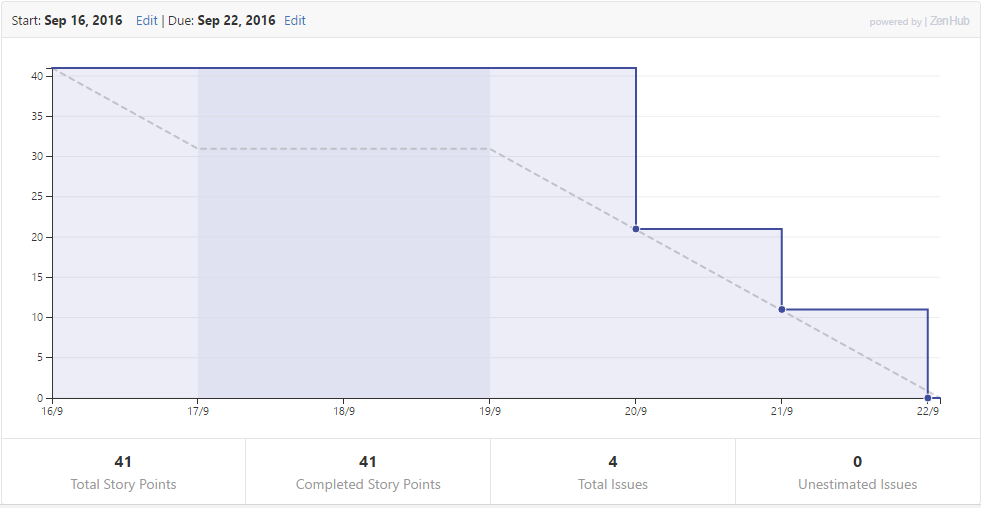
\includegraphics[width=0.99\textwidth]{Semana1}
\caption{Burndown del sprint 1}
\label{fig:A.2.1}
\end{figure}

\subsection{Sprint 2 (22/9/2016 - 30/9/2016)}
En la semana dos vamos a abarcar puntos de la interfaz y puntos de la documentación del proyecto y las tareas son:
 
\begin{itemize}
\item Documentación. 
\begin{itemize}
	\item Aspectos relevantes. 
	\item Técnicas y herramientas.
	\item Planificación temporal.
	\end{itemize}
\item Listas en la interfaz gráfica (Usar tablas para mostrar las rectas que hemos añadido manualmente).
\item Cargar imágenes con el file chooser.
\end{itemize}

\subsubsection{Cumplido:}
Hemos cumplido los objetivos aunque mas adelante y después de una revisión seguramente tengamos que modificar algunas cosas, añadir mas documentación ya que es la primera semana de documentación del proyecto.

Respecto al punto de la tabla donde aparezcan las listas de líneas que vamos añadiendo queda preguntar, si vendría bien añadir tres botones mas al modo manual.

Cosa que en la reunión con el Cliente (Rebeca Garcia \cite{Rebeca:garcia})\footnote{ Dra. Rebeca García González \cite{ubu:Rebe},  que estudia paleobiología y paleoecología de homínidos en la Universidad de Burgos} voy a exponer y posteriormente si parece bien desarrollar.

En cuanto al punto de cargar las imágenes con un \textit{file chooser} de paso, como me sobró algo de tiempo añadí una pantalla de inicio con un mensaje, así la primera vez que abramos la herramienta no se muestren tablas vacías ni una imagen predefinida.

Opte por hacer usar una pagina de inicio a modo de fachada y cuando se cargue la imagen ya iniciar todas las funcionalidades de la aplicación.
En la figura~\ref{fig:A.2.2} se muestra el gráfico del Sprint 2.
\begin{figure}[h]
\centering
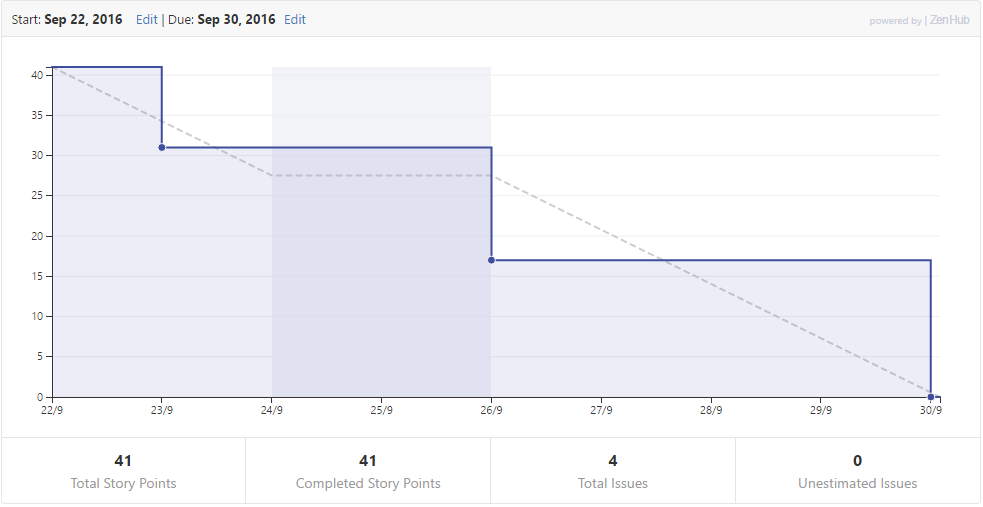
\includegraphics[width=0.99\textwidth]{Semana2}
\caption{Burndown del sprint 2}
\label{fig:A.2.2}
\end{figure}

\subsection{Sprint 3 (30/9/2016 - 7/10/2016)}
En la semana tres vamos a abarcar puntos de la interfaz GUI , generar el informe, y pasar actualizar  el código de PyQt4 a PyQt5 y las tareas son:

\begin{itemize}
	\item Acabar la GUI.
		\begin{itemize}
			\item Mostrar todas las líneas en la tabla.
			\item Poder borrar la línea seleccionada.
		\end{itemize} 
	\item Informe.
		\begin{itemize}
			\item Calcular estadísticas.
			\item Mirar documentación Python.
		\end{itemize}
	\item Pasar código de PyQt4 a PyQt5.
\end{itemize}
\subsubsection{Cumplido:}
Hemos finalizado los objetivos de esta semana y hemos generado funcionalidad a la tabla para agregar las líneas, también añadido que se ilumine la línea seleccionada dentro de la imagen en color amarillo. Hemos añadido funcionalidad para borrar la línea que tenemos seleccionada y también para poder limpiar la tabla completa.

Respecto a la tarea del informe, hemos calculado los estadísticos de todas las líneas, también su clasificación y escritura dentro de un fichero CSV, también la generación de una tabla \LaTeX que se actualiza a cada ejecución con los datos que han salido para poder pegarla fácilmente a un informe.

Como nos dimos cuenta que la versión de PyQt se había actualizado de la cuatro a la cinco pues hemos pasado el código a la nueva version y no ha sido muy difícil.

En la figura~\ref{fig:A.2.3} se muestra el gráfico del Sprint 3.

\begin{figure}[h]
\centering
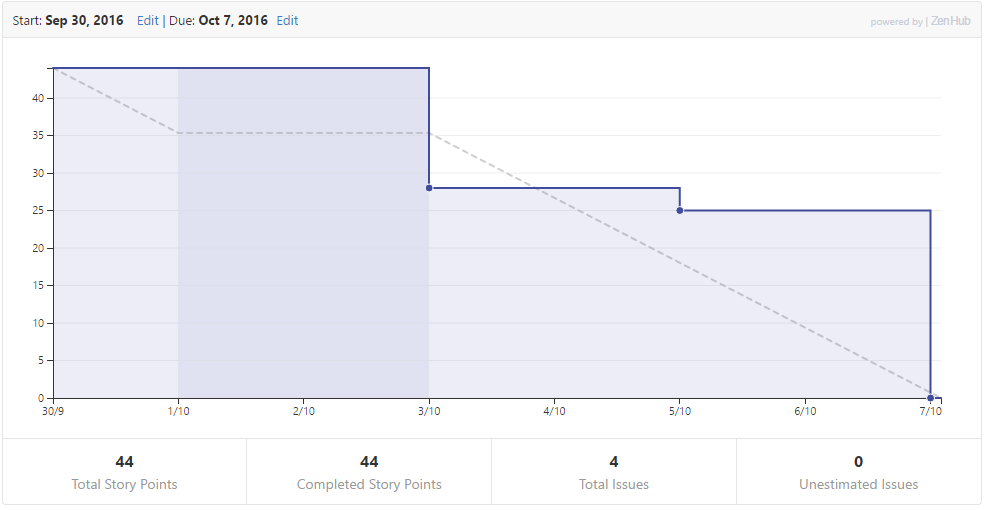
\includegraphics[width=0.99\textwidth]{Semana3}
\caption{Burndown del sprint 3}
\label{fig:A.2.3}
\end{figure}


\subsection{Sprint 4 (7/10/2016 - 14/10/2016)}
En esta semana vamos a abarcar el diseño software de la aplicación así como sacarlo de los NoteBooks y pasarlo a un IDE en condiciones con su subdivisión en clases y paquetes y las tareas son:
\begin{itemize}
	\item Diseño de la aplicación.
		\begin{itemize}
			\item Diagrama de clases.
			\item Diagrama de paquetes.
		\end{itemize}
		
	\item Implementación del código.
		
	\item Corrección de las memorias.
	
	\item Herramienta SonarQube.
	\begin{itemize}
		\item Ejecutar la aplicación.
		\item Corregir las horas de débito.
	\end{itemize}
\end{itemize}
\subsubsection{Cumplido:}
Hemos finalizado los objetivos del sprint.
En paralelo hemos implementado el diseño y el código a medida que teníamos una parte del diseño, de forma incremental, por lo que no se queda del todo reflejado cuando cerramos las tareas.\\

Hemos elegido Eclipse como IDE junto con su plugin PyDev para Python.

La división en clases hemos conseguido tener una primera estimación de como estaba la aplicación.
Respecto a la herramienta SonarQube hemos corregido todos los errores y defectos que salían, a mencionar que no había código repetido ni errores graves.

También detectamos un Bug y fue corregido:
Al mostrar las imágenes, tenia un fallo, consistía en que la imagen estaba como si viéramos su reflejo en un espejo, porque el eje de las << $y$ >> debe ir inverso a como lo conocemos, en vez de << $0-tam-Image$ >> debía ir de << $tam-Imagen-0$ >>.

En la figura~\ref{fig:A.2.4} se muestra el gráfico del Sprint 4.

\begin{figure}[h]
\centering
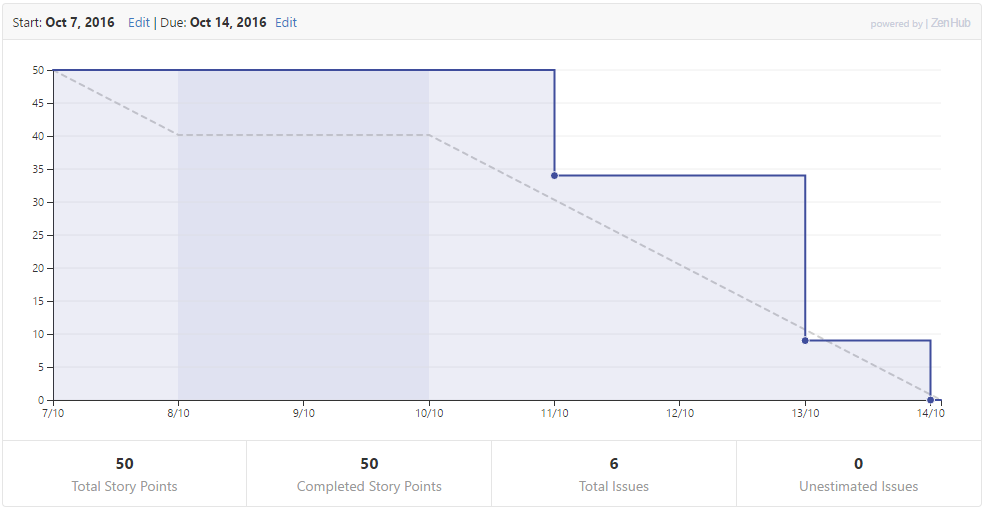
\includegraphics[width=0.99\textwidth]{Semana4}
\caption{Burndown del sprint 4}
\label{fig:A.2.4}
\end{figure}

\subsection{Sprint 5 (13/10/2016 - 22/10/2016)}
Esta semana vamos a continuar con el diseño de la aplicación aplicar los patrones correspondientes y paquetes de las clases.

\begin{itemize}
	\item Aplicar patrones de diseño
	\begin{itemize}
		\item Fachada.
		\item Mediador.
		\item Comando.
	\end{itemize}
	\item Documentar sobre los patrones usados.
	\item XML mirar documentación sobre ello.
\end{itemize}
\subsubsection{Cumplido:}
Esta semana, hemos finalizado los objetivos, hemos documentado los patrones y decidido que con el mediador ya nos servia y el fachada como entrada a la aplicación.
 
El patrón comando en Python no le hemos visto mucho sentido ya que en Python el connect con la función se hace en una sola linea por lo que no hace falta utilizar un patrón comando.

Respecto al XML hemos mirado documentación y lo hemos implementado que guarde los nombres de todos los archivos que generan un proyecto.

En la figura~\ref{fig:A.2.5} se muestra el gráfico del Sprint 5.

\begin{figure}[h]
\centering
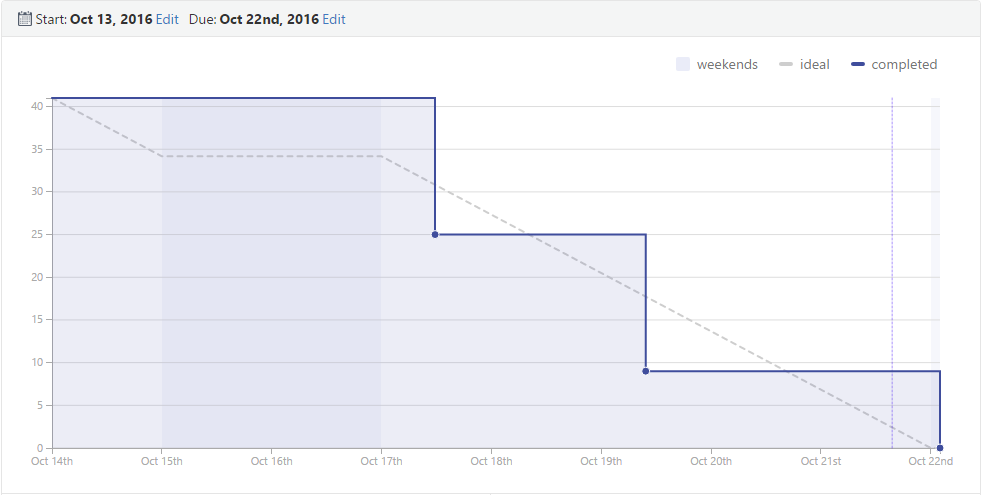
\includegraphics[width=0.99\textwidth]{Semana5}
\caption{Burndown del sprint 5}
\label{fig:A.2.5}
\end{figure}
\subsection{Sprint 6 (22/10/2016 - 28/10/2016)}
Esta semana vamos a intentar ir terminando las tareas para poder la semana que viene tener un prototipo entregable de la aplicación.

\begin{itemize}
\item Completar menús de la GUI.
	\begin{itemize}
		\item Guardar.
		\item Cargar.
		\item Acerca de.
		\item Ayuda.
	\end{itemize}
\item Completar documentación de los fuentes.
	\begin{itemize}
		\item Paquete código.
		\item Paquete gui.
	\end{itemize}
\item Pruebas unitarias.
	\begin{itemize}
		\item Test paquete código.
		\item Test paquete gui.
	\end{itemize}
\end{itemize}
\subsubsection{Cumplido:}
Esta semana, hemos finalizado los objetivos, aunque en el gráfico no queda reflejado por el ataque del día 21 de octubre de 2016 \cite{wiki:Dyn} no pude cerrar las tareas del anterior sprint ni crear las de este.
Respecto a los menús de la gui, hemos añadido y renombrado los campos.

Las funcionalidades añadidas son:
Poder guardar los cambios, podamos abrir y modificar un proyecto, el acerca de y el botón sobre el que va a colgar la ayuda.
También hemos documentado los métodos de las clases del código fuente Python para poder generar la documentación automática con PyDoc.

También hemos desarrollado las pruebas unitarias de la aplicación de todas aquellas funciones que se podía comprobar. 


En la figura~\ref{fig:A.2.6} se muestra el gráfico del Sprint 6.

\begin{figure}[h]
\centering
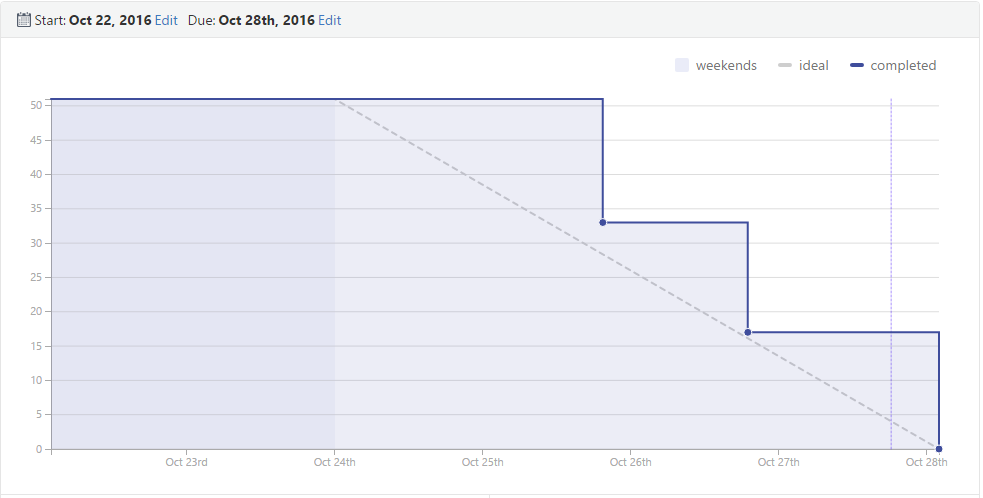
\includegraphics[width=0.99\textwidth]{Semana6}
\caption{Burndown del sprint 6}
\label{fig:A.2.6}
\end{figure}

\subsection{Sprint 7 (28/10/2016 - 04/11/2016)}

Esta semana vamos a añadir funcionalidades para que el usuario tenga mas comodidad al usar la aplicación, evitando que pueda cometer errores o falsos positivos.


\begin{itemize}
	\item Detectar y calcular la referencia.
		\begin{itemize}
			\item Detectar la referencia.
			\item Calcular cuanto es la referencia.
		\end{itemize}
	\item Detectar la región pintable.
	\item Revisar toda la aplicación.
		\begin{itemize}
			\item Revisar el código con SonarQube.
			\item Ajustar los cálculos en algunos puntos.
			\item Añadir botón de cerrar.
		\end{itemize}
	\item Corregir la documentación.
		\begin{itemize}
			\item Memorias.
			\item Anexos.
		\end{itemize}			
\end{itemize}
\subsubsection{Cumplido:}
Esta semana, hemos finalizado todos los objetivos que nos habíamos propuesto, también hemos documentado bastante, no solo corregir lo que teníamos planteado.

El gráfico de esta semana se ha quedado muy desplazado hacia la derecha, porque hemos echo unas pruebas en ZenHub y al sacar varias tareas que ya estaban en cerradas, se ha despintado de la gráfica, pero todas ellas fueron terminadas en tiempo.

Las funcionalidades añadidas son:
\begin{itemize}
	\item Detectar la región pintable: Era uno de los puntos que nos faltaban, para poder conseguir que solo se pudieran pintar, a mano, las lineas dentro del cuadrado pintado por el usuario, en las imágenes. Porque solo esta permitido para este estudio las lineas que se encuentran dentro del recuadro en la imagen.
	\item Detectar y calcular la referencia: En las imágenes de microscopio, se les hace una marca con los aumentos con los que se han echo las imágenes, la referencia, que marca la escala y otros datos importantes.
	Nuestro trabajo ha sido detectarlo y calcular cuantos píxeles son.
	
	\item Hemos añadido el botón de cerrar la aplicación que era un punto en el que aun no habíamos pensado y es necesario.
	
	\item La mejora de la calidad del software pasando la herramienta SonarQube para corregir las posibles mejoras que nos proponga dicha herramienta. 
\end{itemize}

En la figura~\ref{fig:A.2.7} se muestra el gráfico del Sprint 7.

\begin{figure}[h]
\centering
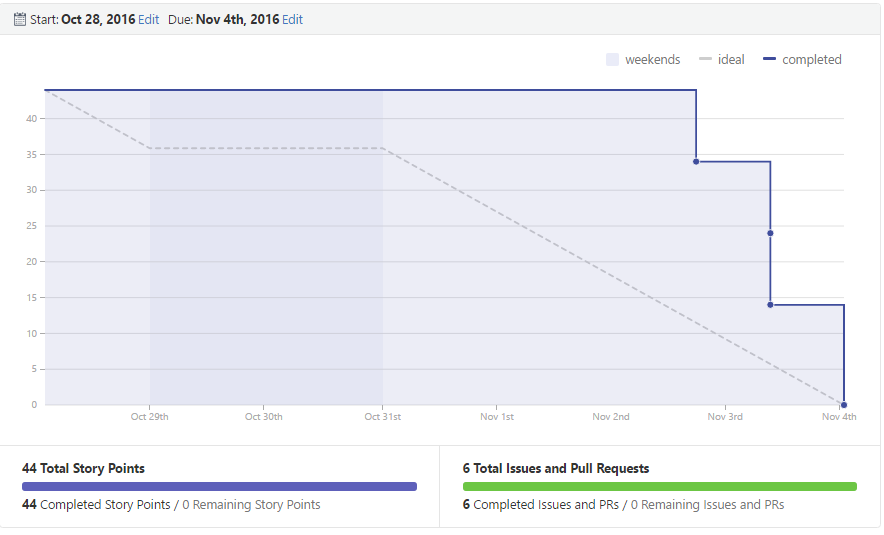
\includegraphics[width=0.99\textwidth]{Semana7}
\caption{Burndown del sprint 7}
\label{fig:A.2.7}
\end{figure}

\subsection{Sprint 8 (04/11/2016 - 11/11/2016)}
Esta semana, va a consistir en investigar sobre el modo automático, dar valor al código en cuanto a calidad aplicando algún concepto de patrones de diseño, haciendo una fachada para la entrada salida.

\begin{itemize}
	\item Diseño:
		\begin{itemize}
			\item Desacoplar del mediador lo que debe ir en la fachada.
			\item Comprobar que los mediadores solo interfieren con aspectos de la GUI.
		\end{itemize}	
	\item Añadir Configuraciones al cálculo.
		\begin{itemize}
			\item Añadir las repeticiones.
			\item Añadir la longitud mínima para filtrar rectas.
		\end{itemize}
		\item Investigación detección de bordes por procesado
			\begin{itemize}
				\item Vamos a usar todos los algoritmos y métodos disponibles en las librerías.
				\item Programar otros conocidos pero que no existan en la librería.
				\item Buscar mucha mas información sobre los metodos conocidos para detección de bordes.
			\end{itemize}					
		\item Investigación detección de bordes por Deep Learning \cite{wiki:deep} \footnote{Conjunto de algoritmos de aprendizaje que modela abstracciones en datos, usando transformaciones no lineales}.
			\begin{itemize}
				\item StrudturedForest.
				\item Retina-Unet. 
			\end{itemize}
\end{itemize}
\subsubsection{Cumplido:}
En esta semana, hemos finalizado los objetivos, además de buscar información sobre los métodos hemos creado un notebook con las pruebas de las ejecuciones de todos ellos.

La semana pasada implementamos la configuración, pero estaba en el código, no podía el usuario cambiarlo en función de sus necesidades.
Por lo que hemos extraído esa parte a la interfaz gráfica, así puede modificar los valores de configuración, guardarse en el XML, para cuando se cargue el proyecto, también se carguen esos valores.

En la figura~\ref{fig:A.2.8} se muestra el gráfico del Sprint 8.

\begin{figure}[h]
\centering
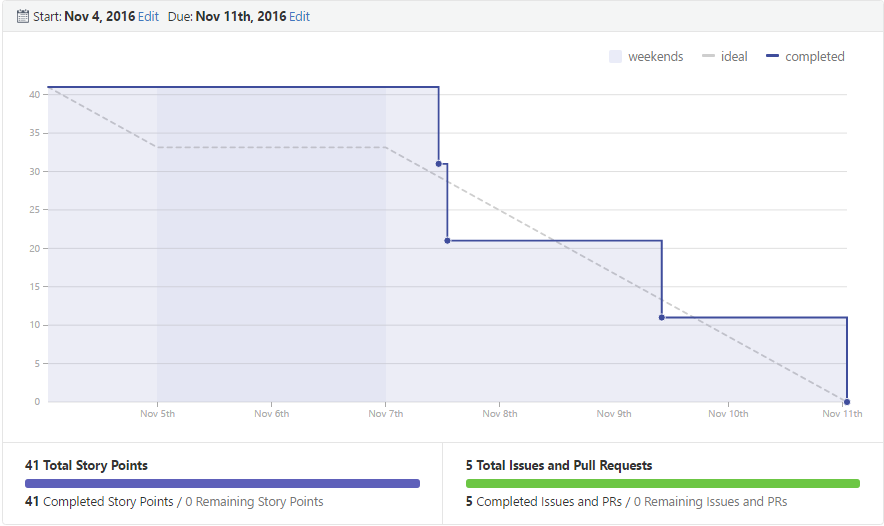
\includegraphics[width=0.99\textwidth]{Semana8}
\caption{Burndown del sprint 8}
\label{fig:A.2.8}
\end{figure}

\subsection{Sprint 9 (04/11/2016 - 11/11/2016)}

Esta semana, vamos a centrarnos en ejecutar y probar todos los métodos estudiados en la semana anterior, algunas modificaciones para facilitar al usuario, su simplicidad y mejorar, los posibles escenarios de ejecución.


\begin{itemize}
	\item Extracción de características.
		\begin{itemize}
			\item Aplicar Hough con valores ajustados.
			\item Extraer y procesar los segmentos.
		\end{itemize}
	\item Investigar y probar Deep Learning para Python 2.7.
		\begin{itemize}
			\item Probar en Python 2.7 ya que en 3.5 no funcionan los algoritmos.
		\end{itemize}
	\item Ejecutable sin dependencias.
		\begin{itemize}
			\item Crear un .exe pero no ha sido posible ya que no hay versiones actuales de esas herramientas para Python 3.5
			\item Crear una alternativa.
		\end{itemize}
	\item Documentar.
		\begin{itemize}
			\item Documentar Memorias. 
			\item Documentar Anexos.
		\end{itemize}
	\item Independencia del color.
		\begin{itemize}
			\item Modificar la distancia al color para que funcione con todos los colores.
		\end{itemize}
\end{itemize}

\subsubsection{Cumplido:}
Esta semana hemos finalizado los objetivos, pero no todo ha sido posible su implementación o realización.
Los algoritmos de Deep Learning, no hemos sido capaces de ejecutarlos, ya que están bastante desactualizados y las dependencias, no están demasiado claras, su ejecución no ha sido posible.

Todos los demás puntos del sprint, han sido realizados con éxito.
La parte de la independencia del color, nos ha permitido que ahora nuestra aplicación, funcione para todas las líneas indiferentemente, del color en el que estén pintadas, el usuario elije que color tienen y las busca.

Respecto a la extracción de características, del modo automático por procesado, hemos conseguido que sea decente partiendo de que las lineas no son fácilmente detectables y las que están mas marcadas no son las que nos interesan.

Para el ejecutable sin dependencias las opciones de crear el .exe no han sido posibles dada la desactualización de las herramientas destinadas a estos fines.
Como alternativa hemos creado una distribución de Miniconda especifica para nuestro propósito que solo contendrá las librerías necesarias para ello.

En la figura~\ref{fig:A.2.9} se muestra el gráfico del Sprint 9.

\begin{figure}[h]
\centering
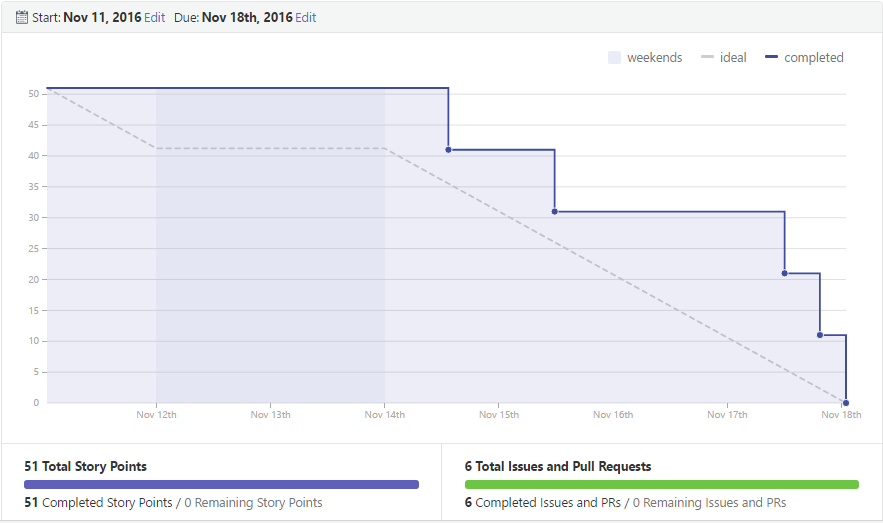
\includegraphics[width=0.99\textwidth]{Semana9}
\caption{Burndown del sprint 9}
\label{fig:A.2.9}
\end{figure}


\subsection{Sprint 10 (18/11/2016 - 25/11/2016)}


\section{Estudio de viabilidad}

\subsection{Viabilidad económica}
En este punto, vamos a hacer es un estudio de viabilidad económica del proyecto, vamos a analizar los gastos que hubiera supuesto, si fuese un proyecto real, para una empresa, en cuanto a tiempo de programación e infraestructura necesaria para ello.


\subsection{Viabilidad legal}
En este punto, lo que vamos a hacer es analizar las librerías que hemos usado, en nuestro proyecto. Buscar los tipos de licencias que tienen cada uno, luego analizar, dependiendo de las compatibilidades, que tipos de licencia podemos aplicar nuestro proyecto y seleccionar uno de ellos.

\begin{table}[]
	\centering
	\caption{Tabla de librerias y sus licencias}
	\label{tabla:Licencias}
	\begin{tabular}{l l l l}
	\hline
	Librería     & Versión & Descripción                                                     & Licencia                \\ 	\hline
	Jinja2       & 2.8     &  \begin{tabular}[c]{@{}l@{}}Un motor de plantillas escrito\\ en Python. \end{tabular}               & BSD                     \\ 	
	Numpy        & 1.11.1  & \begin{tabular}[c]{@{}l@{}}Procesamiento de arrays para\\ números,strings,records y objetos.\end{tabular} & BSD                     \\ 	
	Scipy        & 0.18.1  & Librería científica para Python.                                & BSD                     \\ 	
	Scikit-image & 0.12.3  & \begin{tabular}[c]{@{}l@{}}Librería para tratamiento\\ de imágenes para SciPy.\end{tabular}	               & BSD                     \\ 	
	Networkx     & 1.11    & \begin{tabular}[c]{@{}l@{}}Librería Python para crear y\\ analizar redes complejas.\end{tabular}          & BSD                     \\ 	
	Pillow       & 3.3.1   & \begin{tabular}[c]{@{}l@{}}Librería Python para\\ tratamiento de imágenes.\end{tabular} & \begin{tabular}[c]{@{}l@{}}PIL license\\ similar MIT\end{tabular} \\ 
	Pyqt         & 5.6.0   & Librería Python para crear GUI.                                 &\begin{tabular}[c]{@{}l@{}} GPLv2 o\\ GPLv3\end{tabular}           \\ 
	Matplotlib   & 1.5.3   & \begin{tabular}[c]{@{}l@{}}Librería Python para mostrar\\ gráficos 2D.\end{tabular}                      & PSF-based               \\ 
	Tesseract    & 3.02    & Ocr para ejecutar en Windows.                                   & Apachev2                \\ \hline
\end{tabular}
\end{table}


BSD de tres clausulas es compatible con GLP (esto esta en construcción)


\apendice{Especificación de Requisitos}

\section{Introducción}

Este anexo contendrá los objetivos de la aplicación y los requisitos que va a tener esta.
Consistirán en breves descripciones de todos los objetivos principales, como se subdividen en objetivos mas cortos para conseguir realizarlos y las funcionalidades implementadas.

Requisitos: Contendrá el que consiste el proyecto y las definiciones de los requisitos y objetivos.

\section{Objetivos generales}
\label{txt:objetivos}

Los objetivos que buscamos con este proyecto son:

\begin{itemize}
\item Construcción del prototipo de procesado de las imágenes:
Con este prototipo la funcionalidad buscada era, hacer las pruebas sobre el código, que mas adelante introduciríamos en la aplicación real, pero así podríamos ajustar los parámetros para que funcionase bien. También de esta forma estaríamos seguros que el proyecto es realizable.

\item Construcción de la aplicación: 
Una vez que tengamos el prototipo funcionando, tendríamos que construir una aplicación para ejecutar de una forma mas profesional que simplemente desde un notebook, esto es algo muy avanzado para un usuario sin experiencia, así facilitar la ejecución sin necesidad de depender del notebook.

\item  Construcción del prototipo para el modo automático:
Como hemos realizado el trabajo en tiempo, hemos optado por acoplar un modo de detección de bordes automatizado, para ver si eramos capaces de detectar los segmentos que detectaría un humano.
El problema de este modo es que algunos segmentos no son casi perceptibles por un humano por lo tanto los que estén mas marcados son los que podremos detectar.

\item Añadir el modo automático a la aplicación: 
Como hemos echo anteriormente con el modo de detección de las lineas pintadas. Esta vez también lo acoplaremos a nuestra aplicación, facilitando la ejecución y aplicación de este modo sobre imágenes que no estuvieran pintadas.
\end{itemize}



\section{Catalogo de requisitos}
El proyecto consiste en:
\begin{itemize}
	\item Construcción del prototipo de procesado de las imágenes.
		\begin{itemize}
			\item Lectura de imagen.
			\item Binarización para detectar las pintadas.
			\item Procesado de la imagen binaria.
			\item Extracción de características.
			\item Procesado de las características.
		\end{itemize}
	\item Construcción de la aplicación.
		\begin{itemize}
			\item Lectura de imágenes y cargar en el panel.
			\item Construcción del panel de pestañas
			\item Construcción del modo de automático para lineas pintadas.
			\item Construcción del modo manual para corregir los errores o editar las lineas que hemos pintado.
			\item Construcción de la pestaña para el modo completamente automático.			
		\end{itemize}
	\item Construcción del prototipo para el modo automático.
		\begin{itemize}
			\item Lectura de la imagen.
			\item Equalizacion de la imagen para distribuir el histograma.
			\item Binarización para extraer bordes.
			\item Procesado de la imagen binaria para limpiar de ruido.
			\item Calculo de las características de la imagen.
			\item Procesado de características.		
		\end{itemize}
\end{itemize}


\section{Especificación de requisitos}
\begin{itemize}
	 
\item RF1: Construcción de la aplicación de forma gráfica.
	\begin{itemize}
		\item RF1.1: Construcción de los menús donde mostrar las opciones disponibles en la aplicación.
		\item RF1.2: Construcción del panel de pestañas donde estarán las opciones para los diferentes modos de la aplicación y sus funcionalidades
		\item RF1.3: Construcción del panel donde se mostrara la imagen junto con una barra de opciones con información de la imagen y botones de acciones sobre la imagen.
		\item RF1.4: Lectura de la imagen y cargar en el panel.
	\end{itemize}

\item RF2: Construcción del modo para calcular las estrías pintadas en las imágenes.
	\begin{itemize}
		\item RF2.1: Seleccionar el color de las estrías pintadas que queremos detectar.
		\item RF2.2: Seleccionar la orientación de la imagen,la longitud mínima que debe ignorar y el numero de repeticiones que quiere para calcular los segmentos.
		\item RF2.3: Pedir a la aplicación que use el algoritmo implementado para la detección de las estrías pintadas.			 
		\item RF2.4: Mostrar los segmentos que ha calculado con el algoritmo en el panel donde se muestra la imagen.
	\end{itemize}

\item RF3: Construcción del modo manual para corregir los errores o editar las lineas que hemos pintado.
	\begin{itemize}
		\item RF3.1: Pintar lineas sobre la imagen, pero solo sobre el cuadrado, para añadir nuevos segmentos.
		\item RF3.2: Añadir las lineas que ha calculado el algoritmo de detección de estrías pintadas.
		\item RF3.3: Borrar y limpiar la tabla de los segmentos obtenidos, que se corresponden con las estrías.
		\item RF3.4: Pintar, permitir mover y fijar el cuadrado donde queremos pintar las estrías manualmente.
		\item RF3.5: Guardar los segmentos y obtener las estadísticas y mediciones de todos los segmentos que ha calculado el algoritmo y se muestran en la tabla.			
	\end{itemize}
			 
\item RF4: Construcción del modo completamente automático para detectar las estrías en imágenes sin pintar.
	\begin{itemize}
		\item RF4.1: Seleccionar la orientación de la imagen y la longitud mínima que debe ignorar para calcular los segmentos. 
		\item RF4.2: Mandar calcular al algoritmo las estrías que contiene la imagen.
		\item RF4.3: Mostrar los segmentos que ha calculado con el algoritmo en el panel donde se muestra la imagen.					
		\item RF4.4: Pintar, permitir mover y fijar el cuadrado donde queremos quedarnos con las estrías.
	\end{itemize}
\end{itemize}					

\subsection{Diagrama de casos de uso}
El diagrama que contiene los caso de uso de nuestra aplicación estará contenido en la figura \ref{fig:diagramCasosUso}.	



\begin{figure}[h]
\centering
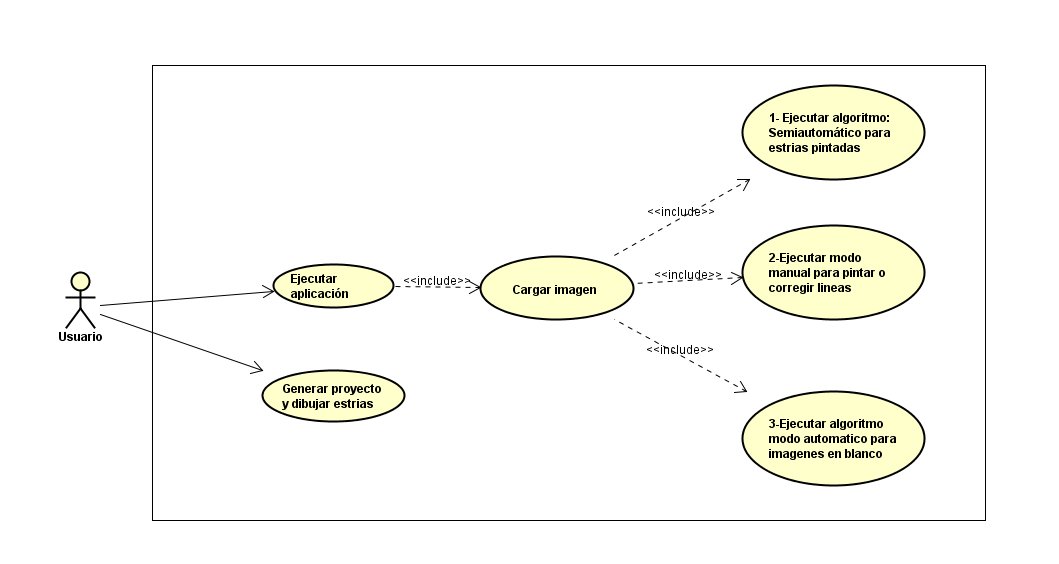
\includegraphics[width=.99\textwidth]{DiagramCasosUso}
\caption{Diagrama de casos de uso.}
\label{fig:diagramCasosUso}
\end{figure}
 
\subsection{Casos de uso}
Las tablas de los casos de uso se muestran en las siguientes figuras, \ref{fig:tablacaso1}, \ref{fig:tablacaso2},\ref{fig:tablacaso3} y \ref{fig:tablacaso4}.
			 
\begin{figure}[h]
\centering
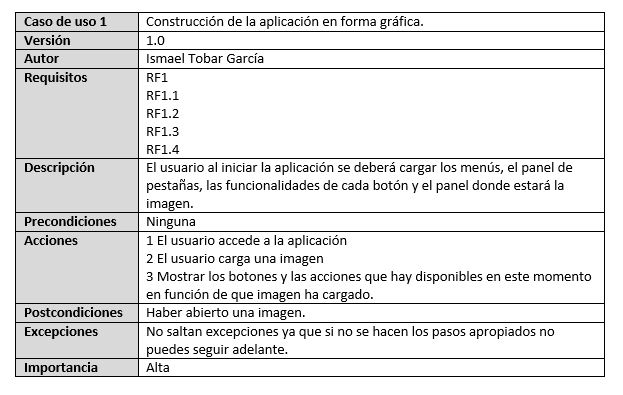
\includegraphics[width=.99\textwidth]{tablacaso1}
\caption{Tabla del caso de uso 1.}
\label{fig:tablacaso1}
\end{figure}

\begin{figure}[h]
\centering
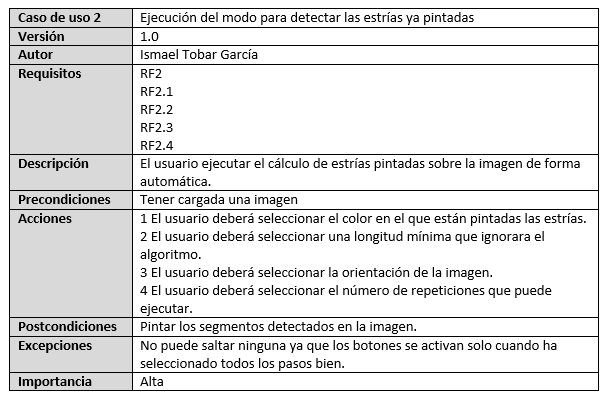
\includegraphics[width=.99\textwidth]{tablacaso2}
\caption{Tabla del caso de uso 2.}
\label{fig:tablacaso2}
\end{figure}

\begin{figure}[h]
\centering
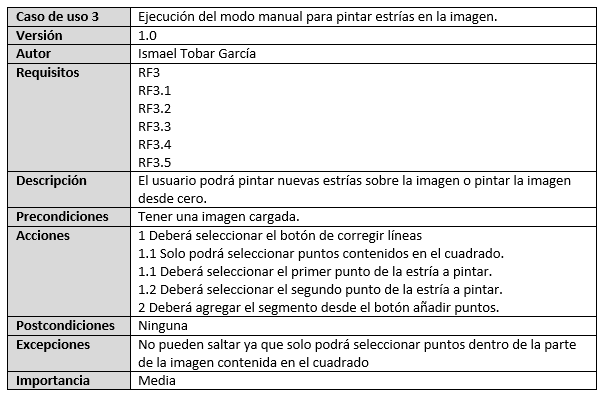
\includegraphics[width=.99\textwidth]{tablacaso3}
\caption{Tabla del caso de uso 3.}
\label{fig:tablacaso3}
\end{figure}

\begin{figure}[h]
\centering
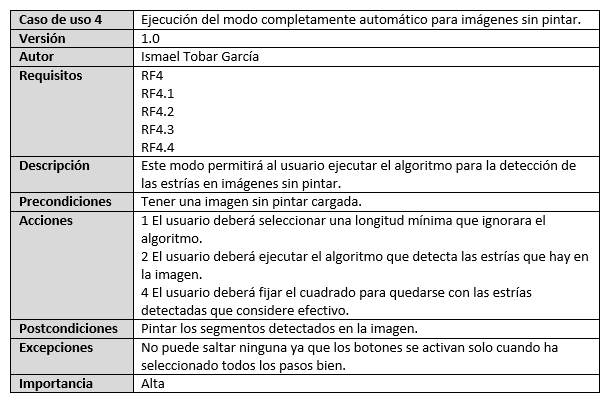
\includegraphics[width=.99\textwidth]{tablacaso4}
\caption{Tabla del caso de uso 4.}
\label{fig:tablacaso4}
\end{figure}

\apendice{Especificación de diseño}

\section{Introducción}

En este apartado vamos a explicar que hemos usado para la resolución del problema en cuanto a herramientas de diseño.

Para la elaboración de los diagramas de paquetes y de clases hemos usado UML como metodología y el programa Astah para implementar los diagramas de clases.

Primero, hemos planeado un prototipo de diseño de cada una de las clases, como podemos observar en la figura~\ref{fig:C.1.1} el diagrama de clases inicial, a medida que las implementábamos las hemos ido completando, para que se correspondieran en lo que finalmente va a quedar.



\section{Diseño de datos}

En este punto vamos a hacer el diseño inicial de las clases de la aplicación y del diseño de paquetes en el que estarán contenidas.

\begin{figure}[h]
	\centering
	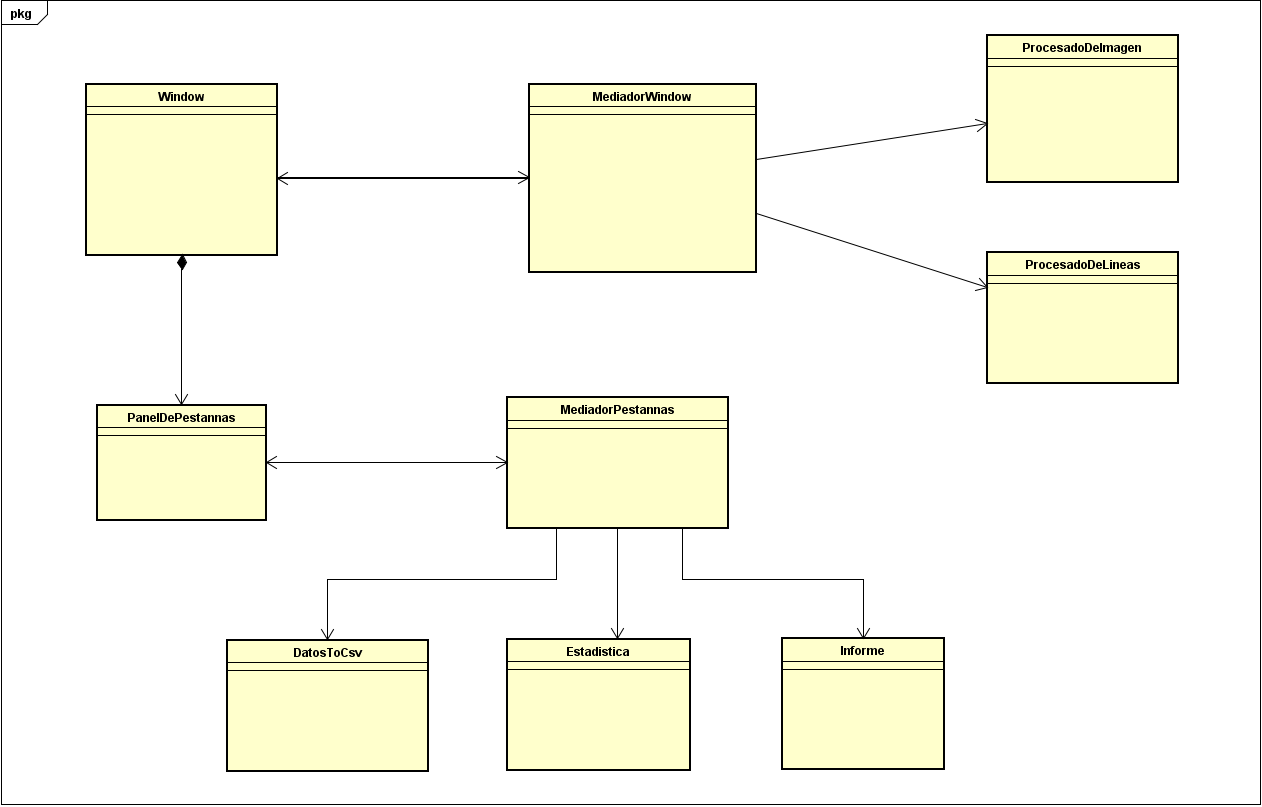
\includegraphics[width=.99\textwidth]{DiaClases}
	\caption{Diagrama de clases inicial}
	\label{fig:C.1.1}
\end{figure}
 

\subsection{Diseño inicial}
\subsubsection{Clases}
En esta parte vamos a hacer una breve descripción del contenido de cada clase y su función.

\begin{itemize}
	\item VentanaInicio: 
Esta clase simplemente hará de fachada entre la ejecución y el acceso a la aplicación real cuando hayamos elegido una imagen que procesar
	\item Window:
Esta clase contendrá la ventana principal, menús, el panel de pestañas y la imagen sobre la que dibujar.
	\item PanelDePestannas:
Esta clase contendrá la botonería y la interacción con la imagen a evaluar.
	\item MediadorPestannas:
Esta clase va a ser un mediador para las pestañas para deslocalizar código y complejidad.
	\item MediadorVentana:
En esta clase va ser un mediador entre la ventana principal y sus métodos para así reducir complejidad en la clase de ventana.
	\item ProcesadoDeImagen:
Esta clase contendrá el tratamiento que tiene que llevar la imagen para la extracción de características a evaluar.
	\item ProcesadoDeLineas:
Esta clase contendrá el procesado de las líneas obtenidas por el procesado de la imagen y el resultado final que obtendremos.
	\item Informe: 
Esta clase contendrá la generación del informe (Tabla) de estadísticas en formato \LaTeX para poder exportar fácilmente a un documento PDF.
	\item DatosToCsv:
Esta clase contendrá el paso de los datos que contiene la tabla a un documento en formato csv del que desde Excel podemos extraer fácilmente los datos.
	\item Estadistica: 
Esta clase contendrá el cálculo de los datos estadísticos y la clasificación de las líneas según su orientación.
\end{itemize}


\subsection{Diseño Final}



\subsection{Diseño de la Interfaz}

\subsubsection{Primera versión}

Para el desarrollo de la interfaz gráfica pensé en una planificación espacial acorde con los elementos que esta contendría.
Un layout que seria muy adecuado podría ser un border layout pero como no existe en PyQt4 lo he tenido que simular gracias a apilar layouts de otros tipos.
Consiguiendo tener una botonería arriba del todo y dos columnas debajo claramente diferenciadas en la que en una estuviera la imagen que vamos a mostrar y en la otra las funcionalidades, como se ilustra en la imagen \ref{fig:5.8}.

\begin{figure}[h]
\centering
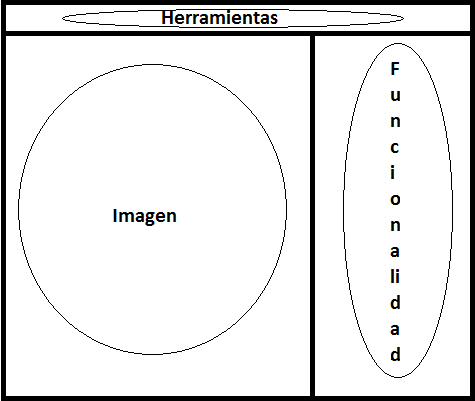
\includegraphics[width=0.65\textwidth]{disenoInter}
\caption{Diseño de la interfaz de usuario}
\label{fig:5.8}
\end{figure}

\subsubsection{Versión a evaluar}

En otro Sprint del proyecto lo que he usado han sido pestañas para así tener en la zona de funcionalidades los modos de trabajo de la aplicación claramente separados, como podemos observar en la figura \ref{fig:5.9}.

\begin{itemize}
\item Detección líneas rojas.
\item Corrección y pintar líneas.
\item Automático.
\end{itemize}


\begin{figure}[h]
\centering
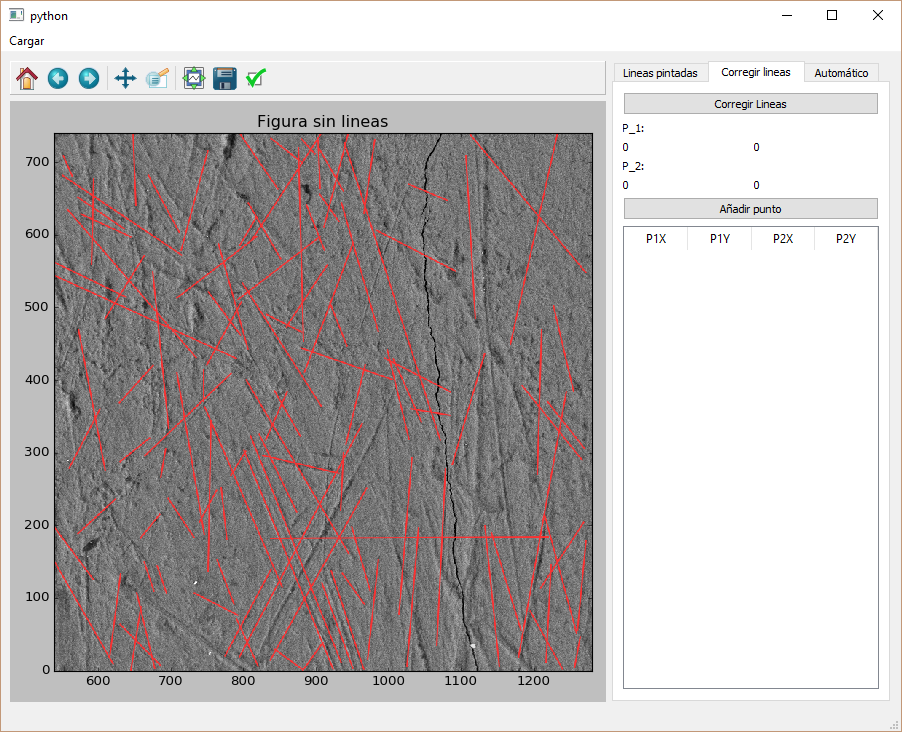
\includegraphics[width=0.99\textwidth]{disenoWi}
\caption{Diseño de la interfaz de usuario}
\label{fig:5.9}
\end{figure}

\textbf{Barra de herramientas}
Es una sección de la interfaz que nos va permitir de momento la carga de imágenes para su procesado \ref{fig:5.10}.
\begin{figure}[h]
\centering
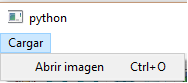
\includegraphics[width=0.35\textwidth]{BarraHerramientas}
\caption{Barra de herramientas de la aplicación}
\label{fig:5.10}
\end{figure}

\textbf{Barra de herramientas de la imagen}
Es una sección de la interfaz que nos permitirá manipular la imagen para realizar estas acciones,como podemos observar en la figura \ref{fig:5.11}.

\begin{itemize}
\item Volver al principio. 
\item Retroceder un paso.
\item Avanzar un paso.
\item Desplazar la imagen.
\item Aumentar la región que seleccionemos.
\item Configurar la región, bordes, etc.
\item Guardar la imagen con su escala.
\item configurar el tamaño y numeración de los ejes.
\item Coordenadas actuales del ratón.
\item Niveles de color de los canales R G B del espacio RGB.
\end{itemize}

\begin{figure}[h]
\centering

\includegraphics[width=0.95\textwidth]{toolbar}
\caption{Barra de herramientas de la imagen}\label{fig:5.11}
\end{figure}


\textbf{FigureCanvas de la imagen}
Es la región donde se muestra la imagen que va a ser ligeramente mas grande que la parte de las pestañas \ref{fig:5.12}.
\begin{figure}[h]
\centering
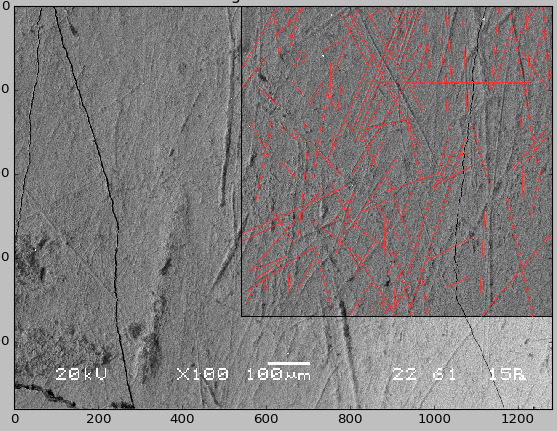
\includegraphics[width=0.65\textwidth]{FigureCanvas}
\caption{FigureCanvas de la imagen}
\label{fig:5.12}
\end{figure}


\textbf{Pestañas}
Sección de la imagen donde estarán implementadas las funcionalidades para visualizar las líneas que son detectadas por el algoritmo. se ilustra en la figura \ref{fig:5.13}.
\begin{itemize}
\item El modo primero es la detección de los surcos en rojo en los dientes 
\item El modo segundo es la corrección/detección manual de las líneas por una persona y quedando reflejadas en la imagen.
\item El modo tercero es la ultima parte del proyecto que consistirá en hacer todo el proceso anterior de forma automática.
\end{itemize}

\begin{figure}[h]
\centering
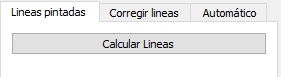
\includegraphics[width=0.65\textwidth]{Pestanas}
\caption{Pestañas}
\label{fig:5.13}
\end{figure}

\section{Diseño procedimental}
En este apartado se van a explicar los pasos que siguen los distintos modos de la aplicación.

\begin{itemize}
	\item Modo semiautomático:
La finalidad de este modo de trabajo en nuestra aplicación, servirá para detectar las estrías que previamente se han pintado en alguna imagen. Para extraer las características de estas.
	\begin{itemize}
		\item Comienza cuando el usuario cargue la imagen en la aplicación.
		\item Posteriormente a la carga, el usuario deberá elegir los parámetros que puede modificar, para la ejecución del algoritmo.
		\item Una vez seleccionados los parámetros, podremos continuar mandando ejecutar a la aplicación el algoritmo, para la detección de las estrías pintadas.
		\item Este nos va a devolver un conjunto de segmentos, que se corresponderán con las estrías que contiene la imagen pintadas, las añadirá a la tabla donde podremos editarlas o añadir algunas que podría no haber detectado dicho algoritmo.
		\item por ultimo podremos guardar las estadísticas, las imágenes original, pintada, longitudes de los segmentos, ángulos, orientaciones, la tabla rellena en formato \LaTeX , para incluir en futuros informes y el fichero de configuración del proyecto.
	\end{itemize}
	\item Modo automático:
	La finalidad de este modo de trabajo de la aplicación, consiste en detectar las estrías de dieta de una imagen en blanco desde el cero. Para extraer características de dichas estrías.
	\begin{itemize}
		\item Primero el usuario deberá cargar una imagen, sin que tenga las estrías pintadas, en la aplicación.
		\item posteriormente, deberá elegir los parámetros disponibles para el modo automático, este consistirá en seleccionar la orientación y la longitud mínima que ignora el algoritmo.
		
		\item Una vez que hayan sido seleccionados se habilitara la función de detección de las estrías. Al ejecutar este algoritmo nos mostrara todas las estrías que detecto en la imagen y nos permitirá mover la región de interés que queremos analizar.
		\item Al mover la región de interés que nos conviene analizar y fijarlo, desechará las estrías que no estén contenidas y también los trozos de las detectadas que se salgan fuera de la región.
		\item Por último, el paso anterior nos mostrara en la tabla de edición de los segmentos las estrías que ha detectado, pudiendo modificar o eliminar aquellas que nosotros no consideremos útiles.
		También nos permitirá guardar el proyecto tal y como estaba para obtener las estadísticas y demás datos relevantes de las estrías detectadas.
	\end{itemize}
	\item Modo manual:
	La finalidad de este modo no es otra mas que poder incluir el factor humano en la aplicación y corregir los posibles errores o modificar ciertas estrías que nuestro algoritmo ha detectado.
	\begin{itemize}
		\item Después de cargar cualquier imagen en la aplicación podremos acceder a las funciones de este modo.
		\item Para pintar desde cero una imagen, sin que tenga estrías, podemos hacer clic en el la pestaña de corregir lineas y mover la región de iteres por la imagen en la zona que queremos pintar. 
		\item Dentro de la pestaña, anteriormente mencionada, en el botón con el mismo nombre al hacer clic, la primera vez fijaremos el cuadrado y procederemos a seleccionar el origen y el final de la estría que queremos detectar, para añadirla simplemente tendremos que hacer click sobre el botón añadir punto y esta quedará incluida en la tabla. Para pintar nuevas estrías en una imagen que ya contenga estrías pintadas procederemos de forma similar, pero no podremos mover la región de interés. 
		\item Una vez que tengamos alguna estría pintada en nuestra imagen podremos proceder a guardar las estadísticas y todos los datos relevantes del proyecto, de forma similar a los otros modos.
	\end{itemize}

\end{itemize}

\section{Diseño arquitectónico}

En esta sección del anexo de diseño, vamos a explicar y mostrar de forma general como esta diseñado el proyecto, en cuanto a la distribución de paquetes y los patrones de diseño que hemos aplicado.

\subsection{Diseño de paquetes inicial}

En este punto vamos a hacer una breve descripción de cada paquete y de su contenido dentro de la aplicación.

\begin{itemize}
\item Gui:
Este paquete contendrá todos los elementos gráficos de la aplicación y todos lo que se corresponde con interacción con el usuario.
	\begin{itemize}
	\item Mediadores:
	Este paquete va a contener los mediadores de la interfaz para deslocalizar código y complejidad en esta.
	\end{itemize}
\item Código: Este paquete contendrá todas las clases de cálculo que necesitará la aplicación:
	\begin{itemize}
	\item Estadísticas:
	Este paquete contendrá las clases del cálculo de estadísticas.
	\item Informes:
	Este paquete contendrá la generación del informe \LaTeX
	\item Procesado:
	Este paquete se va a encargar tanto del procesado de la imagen 			como del procesado de los segmentos extraídos hasta conseguir los 		segmentos finales.
	\end{itemize}
\end{itemize}

\begin{figure}[h]
	\centering
	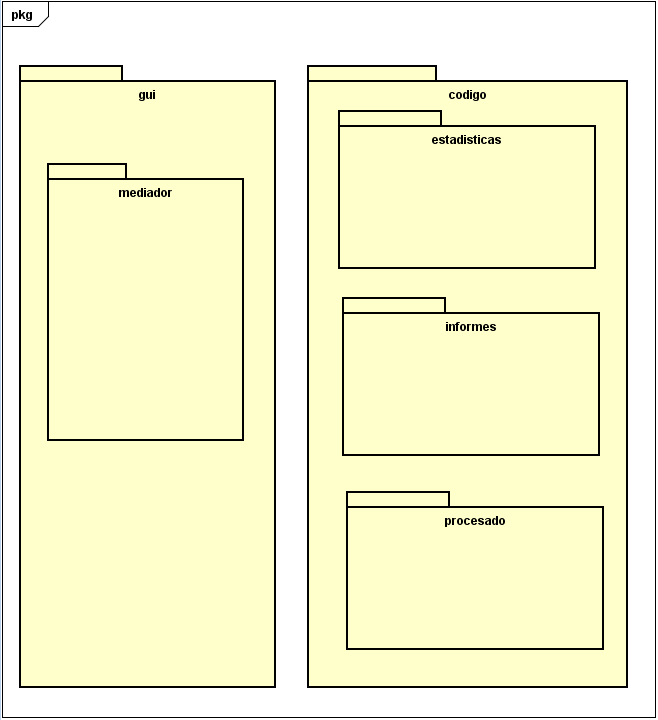
\includegraphics[width=.99\textwidth]{DiaPackages}
	\caption{Diagrama de paquetes inicial}
	\label{fig:C.1.2}
\end{figure}

\subsection{Diseño de paquetes Final}


\subsection{Patrones de diseño}
En este apartado vamos a usar de los patrones de diseño que hemos utilizado en nuestra aplicaron.

El patrón más importante y con el que vamos a empezar es el medidor que consigue hacer que la interfaz este limpia simplemente con las declaraciones de las variables que más adelante va a utilizar.
La base de los patrones de diseño, está explicado en su libro más significativo, el cual es \cite{Hunt2013}.

\begin{itemize}
\item Mediador \cite{wiki:Mediador}: Se utiliza para encapsular las interacciones entre los objetos de la interfaz por lo que se clasifica como patrón de comportamiento.
Como dato curioso, es de los pocos patrones que permiten la bidireccionalidad de comunicación entre las clases, por eso es el patrón idóneo para la interacción de las clases de la interfaz gráfica.
Aplicando este patrón reducimos la dependencia del código por lo que de esta forma las interfaces no ven lo que tienen por debajo y reduce la complejidad.

\textbf{Obtenemos:}
\begin{itemize}
\item Conseguir desacoplamiento.
\item Simplificar y aclarar la comunicación.
\item Centralizar el control.
\item Interfaz simple para un sistema complejo.
\end{itemize}

\item Comando \cite{wiki:Comando}: Se utiliza para encapsular el contenido de una función, así ni el emisor de la operación ni el receptor, sabe que hay por debajo, pero si poder acceder a las funciones que hay.\\\\
\textbf{Obtenemos:}
\begin{itemize}
\item Permitir la parametrización.
\item Visualizar que ordenes se ejecutan en cada paso.
\item Construir operaciones complicadas a partir de otras más sencillas.
\item Permitir saber que habría que hacer para deshacer una operación.
\end{itemize}
\item Fachada \cite{wiki:Fachada}: Es un patrón de diseño estructural, sirve para reducir la complejidad con la división en clases más pequeñas y reduciendo sus dependencias.\\\\
\textbf{Obtenemos:}
\begin{itemize}
\item Separar en niveles la aplicación.
\item Reducir su complejidad.
\item Desacoplar el código.
\item Interfaz simple para un sistema complejo.
\item Potable y reutilizable.
\end{itemize}
\end{itemize}

\apendice{Documentación técnica de programación}

\section{Introducción}
Esta sección está dirigida a otros desarrolladores, de modo que puedan continuar el proyecto y entenderlo. En él se describen en detalle el funcionamiento del proyecto y los aspectos que podrían mejorarse o modificarse en el futuro.
\section{Estructura de directorios}

\subsection{Ejecutables:} 
	\begin{itemize}
		\item EjecutarGui: Este fichero se corresponde con el ejecutable para lanzar la aplicación en modo GUI.
		\item EjecutarTest: Este fichero se corresponde con el ejecutable para lanzar los test de la aplicación en modo consola.
		\item Documentar: Este fichero se corresponde con el ejecutable para documentar la aplicación de forma recursiva y crear los ficheros HTML correspondientes.
	\end{itemize}
		
\subsection{Documentación:}
En esta carpeta está contenida la documentación en formato HTML.
	\begin{itemize}
		\item pydoc: Esta carpeta se corresponde con la documentación de pydoc
	\end{itemize}

\subsection{Src:}
Esta carpeta contiene todos los ficheros de código fuente del proyecto, el OCR, y los test.

\subsubsection{Proyecto:}
Esta carpeta corresponde todos los ficheros de código fuente del proyecto, todos los módulos o paquetes.

\textbf{Análisis}
\begin{itemize}
	\item Estadísticas.
		\begin{itemize}
			\item Estadística.
		\end{itemize}
	\item Informes:
		\begin{itemize}
			\item ConfiguracionToXML.
			\item DatosToCsv.
			\item Informe.
			\item InGuardarDatos
		\end{itemize}
	\item Procesado:
		\begin{itemize}
			\item ProcesadoAutomatico.
			\item ProcesadoDeImagen
			\item ProcesadoDeLineas
		\end{itemize}
	\item Diccionario:
		\begin{itemize}
			\item Diccionario
			\item DiccionarioING
		\end{itemize}
	\item FachadaBotonesAndLayaout.
	\item FachadaEntradaSalida.	
	\item MediadorPestannas.
	\item MediadorVentana.
\end{itemize}	

\textbf{GUI}
\begin{itemize}
		\item PanelDePestannas
		\item PintarRectangulo
		\item VentanaInicio
		\item VisorHtml
		\item Window
\end{itemize}

\subsubsection{Tesseract:}
Esta carpeta contiene el ejecutable del OCR junto con sus ficheros de configuración para poderlo ejecutar.

\subsection{Test:}
Esta carpeta contiene los test del código para comprobar que funcionan correctamente.
\subsubsection{Codigo:}
\begin{itemize}
	\item Estadísticas:
		\begin{itemize}
			\item TestEstadistica
		\end{itemize}
	\item Informes:
		\begin{itemize}
			\item TestConfiguracionToXML
			\item TestDatosToCsv
			\item TestInforme
		\end{itemize}
	\item Procesado:
		\begin{itemize}
			\item TestProcesadoDeImagen
			\item TestProcesadoDeLineas
		\end{itemize}
\end{itemize}

\section{Manual del programador}
En esta sección vamos a describir como se han programado las partes mas importantes que son las que mas nos interesan.
\subsection{Procesado}
Para programar el procesado hemos encadenado sucesivos pasos, que dividiremos en tres secciones.

\begin{itemize}
\item ProcesadoDeImagen: Este se corresponde con el procesado de la imagen para la extracción de las características.
	\begin{enumerate}

	\item Hemos calculado de la imagen la distancia a un color: Se corresponde con el que estén pintadas los segmentos, lo selecciona el usuario. Evitamos cualquier color que hiciese que falle el algoritmo, filtrando la selección por el canal del modelo de color HSV, que indica la saturación. En nuestra imagen lo único que tiene una saturación alta son los segmentos pintados ya que la imagen esta en escala de grises.

	\item Binarizamos la imagen con la distancia al color para obtener la máscara con los objetos que queremos detectar y reducimos el grosor de estos.

	\item Sobre la máscara reducida calculamos los segmentos por la transformada de Hough.
	\end{enumerate}

\item ProcesadoDeLineas: Este módulo contiene el procesado de las lineas, detectadas en el último paso del punto anterior.
\begin{enumerate}

\item Primero de todo, lo que tenemos no son segmentos completos, sino subsegmentos que forman los segmentos reales. Tenemos que unirlos aquellos que sean muy similares, caracterizados por distancia y ángulo.

\item Para realizar la unión lo primero que haremos será ir añadiendo, un camino entre los dos segmentos, a un grafo, de aquellos que cumplan lo anterior.

\item Obtendremos las uno componentes del grafo \footnote{Se explica en las memorias pero podemos encontrarlo aquí también \cite{Wiki:Grafos}}, que se corresponden, con los clusters, que son los segmentos buscados.
\end{enumerate}

\item ProcesadoAutomatico: Este apartado aunque lleva proceso similares a los anteriores no puede ir junto ya que necesita otros pasos intermedios.
\begin{enumerate}

\item Usaremos el detector de bordes que hemos implementado.
\item Ecualizaremos la imagen para distribuir su histograma.
\item Calculamos los autovectores de la matriz Hessiana y nos quedamos con los autovectores largos.
\item Binarizamos la imagen y procesamos dicha imagen. Queda reflejado en anexo \ref{anexo:F}.
\end{enumerate}

\end{itemize}

\subsection{GUI}

\begin{itemize}
	\item Imagen y líneas: Para pintar las imágenes, hemos usado el backend de Matplotlib, que nos muestra la imagen sobre unos ejes de coordenadas, que nos indican e informan sobre las coordenadas de cada pixel. Gracias a esto y a los métodos de conexión sobre los eventos, hemos podido simplificar al máximo la obtención de los puntos, la forma de pintar los segmentos detectados y la interacción de usuario.
	
	\item OCR: Para leer la referencia de la imagen hemos usado un OCR conocido que se llama Tesseract. Le pasamos el recorte de la imagen que contiene la referencia y nos devuelve el numero que contiene.
\end{itemize}

\section{Compilación, instalación y ejecución del proyecto}

\subsection{Compilación:}
En Python no hace falta compilar el proyecto ya que es un lenguaje interpretado. Necesitaremos únicamente tener Python instalado, a través de Miniconda o cualquier otra distribución, de Python.

Python es un lenguaje interpretado y necesitamos tener Python 3.5. junto con las librerías usadas, pero instalar una a una dichas librerías es un trabajo complejo, para un usuario. Por eso para facilitar la instalación de Python hemos optado por usar Miniconda, es una distribución que facilita dicha instalación pero sin ninguna librería instalada, por lo que es mas ligero, 50 Megas, frente a Anaconda, cerca de 500 Megas. Quedando a nuestra disposición indicar que librerías instalar.

En la primera ejecución del código nos va a descargar e instalar todas las librerías que necesitamos.

\subsection{Instalación:}
Para poder ejecutar deberemos instalar Miniconda en 
 \textrm{C\textbackslash Users\textbackslash TuUsuario}, Es el directorio predefinido por Miniconda, una vez que lo tengamos instalado podremos proceder a hacer doble clic sobre el ejecutable  \textrm{EjecutarGui.bat} que instalará las dependencias a las librerías que necesitamos para su ejecución.

\subsection{Ejecución del proyecto:}
Para la primera ejecución, si no tenemos las librerías instaladas, al hacer doble clic sobre EjecucionGui.bat, tardará un rato en descargarlas y crear el entorno virtual de Miniconda con únicamente las librerías que se usan. No obstante, en lo sucesivo únicamente ejecutara la aplicación.

Si la descarga de las librerías se interrumpe por una caída de la red u otro problema, nos dará un error. Pero si volvemos a ejecutar, se iniciará donde se paró la descarga, es decir no perdemos lo que ya haya conseguido descargar.


\subsection{Conclusiones:}
Hemos seguido otras formas de conseguir crear un entorno de ejecución, hemos intentado crear el ejecutable como se detalla en las memorias pero no hemos sido capaces, por problemas de versiones, aun no están disponibles.



\section{Pruebas del sistema}
En esta sección vamos a informar como ejecutar los test que están ubicados en la carpeta Test dentro de la carpeta src del proyecto. 

\subsection{Test Python:}
Dichos test están escritos en Python usando la librería unittest.

Hay muchas comprobaciones sobre las funciones de cálculo y aquellas que escriben y leen ficheros, pero para la parte de la interfaz gráfica no hay hechas pruebas ya que no se puede controlar del todo esta part. Pero ha sido probada por mí y todos los aspectos añadidos y no produce fallos conocidos.

Para ejecutarlos basta con ejecutarlos desde Eclipse, el main de los test mainTest.py o también si preferimos podemos ejecutarlos desde la terminal con el mismo fichero.
Otra opción para ejecutar los test es dar doble clic sobre el ejecutable EjecutarTest que esta en la carpeta de los ejecutables. 

Aparte de los datos proporcionados en la ejecución hemos puesto una salida informativa para cada test y las partes que comprueba.
 
\subsection{Test de calidad}
En este apartado vamos a mostrar las medidas que vamos a usar para conseguir la calidad de las imágenes y explicar las formulas obtenidas de \cite{wiki:confMatrix}.

Para una mejor clasificación y obtener unas medidas tangibles hemos optado por usar la clásica matriz de confusión que diferencia 4 valores como podemos observar en la tabla \ref{tab:ConfMatrix}.

\begin{itemize}
\item True positive rate (TPR): Mide la proporción de los elementos que se han considerado como positivos y son positivos.
\[TPR=\frac{TP}{TP+FN}\]

\item True negative rate (TNR):Mide la proporción de los elementos que se han considerado como negativos y son negativos. 
\[TNR=\frac{TN}{FP+TN}\]

\item Positive predictive value (PPV): Mide la proporción de elementos clasificados como verdaderos positivos entre los positivos.
\[PPV=\frac{TP}{TP+FP}\]


\item Negative predictive value (NPV): Mide la proporción de elementos clasificados como verdaderos negativos entre los negativos.  
\[NPV=\frac{TN}{TN+FN}\]


\item False positive rate (FPR):
Mide la proporción de los elementos que se han considerado como falsos positivos entre los que son negativos reales.
 \[FPR=1-TNR\]

\item False discovery rate (FDR):
Mide la proporción de los elementos que se han considerado como falsos positivos entre los que son positivos de verdad.
\[FDR=1-PPV\]

\item Miss rate or false negative rate (FNR):
Mide la proporción de los elementos que se han considerado como falsos negativos entre los que son  positivos. \[FNR=1-TPR\]

\item Accuracy (ACC): Mide el error observable.
\[ACC=\frac{TP+TN}{P+N}\]

\item Valor F1: Este valor muestra la media armónica entre la precision y la sensibilidad del modelo.
\[F1=\frac{2TP}{2TP+FP+FN}\]

\item Matthews correlation coefficient (MCC):
Esta medida se usa en Maching Learning para medir la calidad de la clasificación en dos clases \cite{wiki:machineMCC}.
 \[MCC=\frac{TP*TN-FP*FN}{\sqrt{(TP+FP)*(TP+FN)*(TN+FP)*(TN+FN)}}\]
 
\item Informedness or Bookmaker Informedness (BM):
Esta medida informa de la generalización de un problema multi-clases y estima la probabilidad de decisión.
 \[BM=TPR+TNR-1\]

\item Markedness (MK):
Esta es la medida de cuando una variable es marcada como predicción o causa posible de otra.
 \[MK=PPV+NPV-1\]


\end{itemize}



\subsubsection{Pruebas}
Aquí van a aparecer una muestra de las pruebas que hemos realizado sobre la aplicación para medir la calidad de la detección.


Para las pruebas vamos a optar por construir una matriz de confusion sobre los resultados, la tabla mostrada a continuación, sera el modelo que vamos a seguir \ref{tab:ConfMatrix}.

\begin{table}
  \begin{center}
    \begin{tabular}{c l c c}
                 &                & \multicolumn{2}{c}{\cellcolor{brown!25}Predicted condition}   \\
                 &                & \cellcolor{brown!15}Positive prediction & \cellcolor{brown!45}Negative prediction \\
       \cellcolor{blue!15}True      & \cellcolor{blue!10}Positive class & \cellcolor{green!25}True positive (TP)  & \cellcolor{red!25}False negative (FN) \\
       \cellcolor{blue!15}Condition & \cellcolor{blue!30}Negative class & \cellcolor{red!25}False positive (FP) & \cellcolor{green!25}True negative (TN)  \\
    \end{tabular}
  \end{center}
  \caption{Estructura de la matriz de confusion.}
  \label{tab:ConfMatrix}
\end{table}



Prueba 1: La matriz de confusión obtenida para esta prueba la podemos observar en la tabla \ref{tab:pruebas}.
Las imágenes original, como muestra la figura \ref{fig:orip1}, y calculada, como muestra la figura \ref{fig:calcp1}, las podemos observar en la figura \ref{fig:p1}.
Los resultados de las medidas de calidad se muestran en la tabla \ref{tab:parte}.

Prueba 2: La matriz de confusión obtenida para esta prueba la podemos observar en la tabla \ref{tab:pruebas}.
Las imágenes original, como muestra la figura \ref{fig:orip2}, y calculada, como muestra la figura \ref{fig:calcp2}, las podemos observar en la figura \ref{fig:p2}.
Los resultados de las medidas de calidad se muestran en la tabla \ref{tab:parte}.

Prueba 3: La matriz de confusión obtenida para esta prueba la podemos observar en la tabla \ref{tab:pruebas}.
Las imágenes original, como muestra la figura \ref{fig:orip3}, y calculada, como muestra la figura \ref{fig:calcp3}, las podemos observar en la figura \ref{fig:p3}.
Los resultados de las medidas de calidad se muestran en la tabla \ref{tab:parte}.

Prueba 4: La matriz de confusión obtenida para esta prueba la podemos observar en la tabla \ref{tab:pruebas}.
Las imágenes original, como muestra la figura \ref{fig:orip4}, y calculada, como muestra la figura \ref{fig:calcp4}, las podemos observar en la figura \ref{fig:p4}.
Los resultados de las medidas de calidad se muestran en la tabla \ref{tab:parte}.




\begin{table}[]
\centering
\caption{Tabla de resultados matriz de confusión}
\label{tab:pruebas}
\begin{tabular}{@{} lrrrr @{}}
\hline
Prueba                & True positive & False negative & False positive & True negative \\ \hline
Figura \ref{fig:p1} & 36136         & 3840           & 3685           & 1185139       \\ \hline
Figura \ref{fig:p2} & 31670         & 844            & 6514           & 1189772       \\ \hline
Figura \ref{fig:p3} & 23114         & 8238           & 7103           & 1190345       \\ \hline
Figura \ref{fig:p4} & 30284         & 1773           & 14753          & 1181990       \\ \hline
\end{tabular}
\end{table}



\begin{table}[]
\centering
\caption{Resultados medidas de calidad}
\label{tab:parte}
\resizebox{\textwidth}{!}{
\begin{tabular}{@{} lllllllllllllll @{}}
\hline
Prueba                & TPR  & TNR  & PPV  & NPV  & FPR   & FDR  & FNR  & ACC  & F1   & MCC  & BM   & MK   \\ \hline
Figura \ref{fig:p1} & 0.90 & 0.99 & 0.99 & 0.99 & 0.003 & 0.09 & 0.09 & 0.99 & 0.91 & 0.90 & 0.9  & 0.90 \\ \hline
Figura \ref{fig:p2} & 0.97 & 0.99 & 0.83 & 0.99 & 0.17  & 0.17 & 0.02 & 0.99 & 0.90 & 0.90 & 0.83 & 0.82 \\ \hline
Figura \ref{fig:p3} & 0.74 & 0.99 & 0.76 & 0.99 & 0.01  & 0.24 & 0.26 & 0.99 & 0.75 & 0.74 & 0.73 & 0.76 \\ \hline
Figura \ref{fig:p4} & 0.94 & 0.99 & 0.67 & 0.99 & 0.01  & 0.33 & 0.05 & 0.99 & 0.78 & 0.79 & 0.93 & 0.67 \\ \hline
Media & 0.88 & 0.99 & 0.81 & 0.99 & 0.04  & 0.20 & 0.11 & 0.99 & 0.84 & 0.83 & 0.85 & 0.78 \\ \hline
Desviación & 0.10 & 0 & 0.13 & 0 & 0.08  & 0.10 & 0.10 & 0 & 0.08 & 0.08 & 0.08 & 0.09 \\ \hline
\end{tabular}
}
\end{table}



\begin{figure}
	\begin{subfigure}[c]{.5\linewidth}
	\centering\large 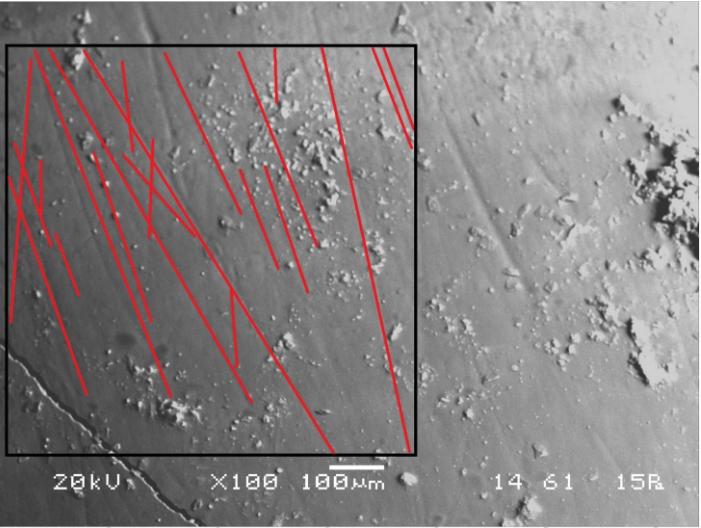
\includegraphics[width=.9\textwidth]{prueba1Ori}
	\caption{Estrías pintadas por el usuario prueba 1.}\label{fig:orip1}
	\end{subfigure}%
	\begin{subfigure}[c]{.5\linewidth}
	\centering\large 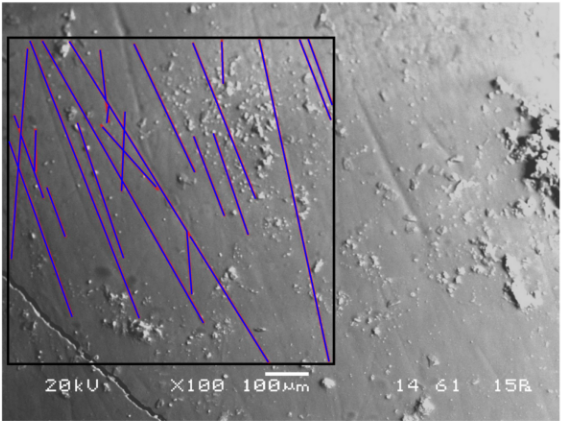
\includegraphics[width=.9\textwidth]{prueba1Detec}
	\caption{Estrías pintadas por la aplicacion prueba 1.}\label{fig:calcp1}
	\end{subfigure}%
	\caption{Imágenes prueba 1}
	\label{fig:p1}
\end{figure}



\begin{figure}
	\begin{subfigure}[c]{.5\linewidth}
	\centering\large 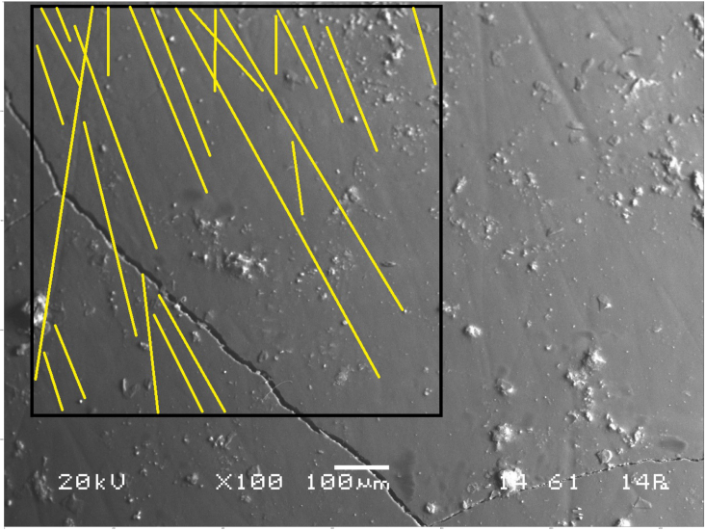
\includegraphics[width=.99\textwidth]{prueba2Ori}
	\caption{Estrías pintadas por el usuario prueba 2.}\label{fig:orip2}
	\end{subfigure}%
	\begin{subfigure}[c]{.5\linewidth}
	\centering\large 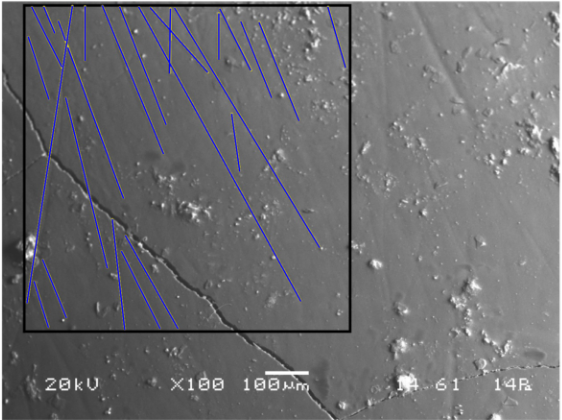
\includegraphics[width=.99\textwidth]{prueba2Detec}
	\caption{Estrías pintadas por la aplicacion prueba 2.}\label{fig:calcp2}
	\end{subfigure}%
	\caption{Imágenes prueba 2}
	\label{fig:p2}

\end{figure}


\begin{figure}
	\begin{subfigure}[c]{.5\linewidth}
	\centering\large 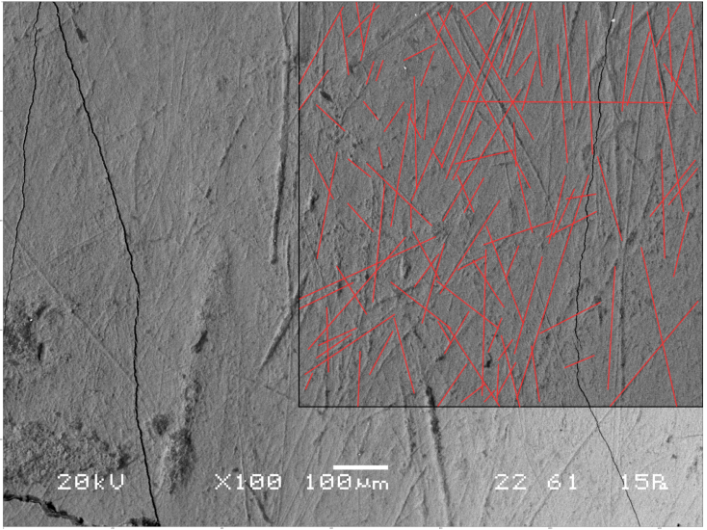
\includegraphics[width=.9\textwidth]{prueba3Ori}
	\caption{Estrías pintadas por el usuario prueba 3.}\label{fig:orip3}
	\end{subfigure}%
	\begin{subfigure}[c]{.5\linewidth}
	\centering\large 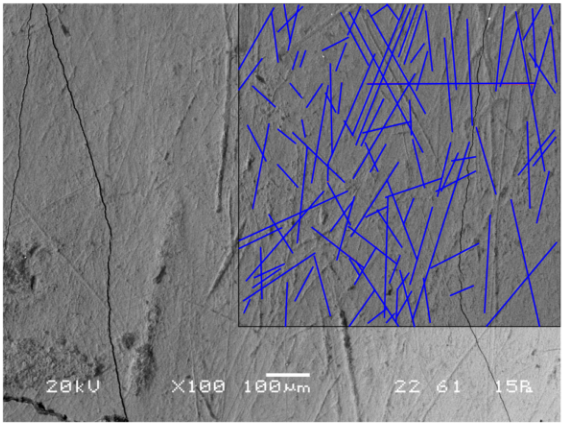
\includegraphics[width=.9\textwidth]{prueba3Detec}
	\caption{Estrías pintadas por la aplicacion prueba 3.}\label{fig:calcp3}
	\end{subfigure}%
	\caption{Imágenes prueba 3}
	\label{fig:p3}

\end{figure}



\begin{figure}
	\begin{subfigure}[c]{.5\linewidth}
	\centering\large 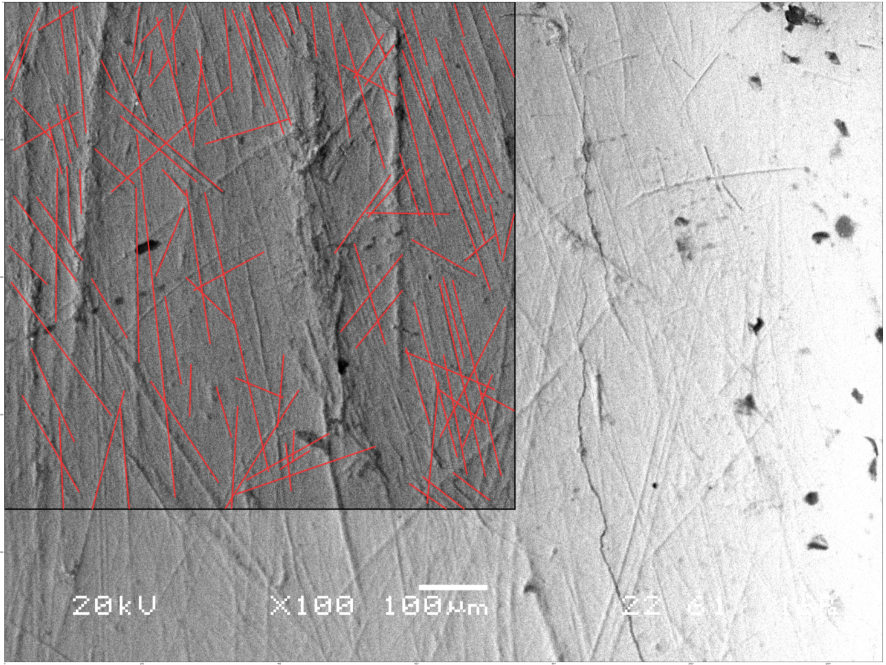
\includegraphics[width=.9\textwidth]{prueba4Ori}
	\caption{Estrías pintadas por el usuario prueba 4.}\label{fig:orip4} 
	\end{subfigure}%
	\begin{subfigure}[c]{.5\linewidth}
	\centering\large 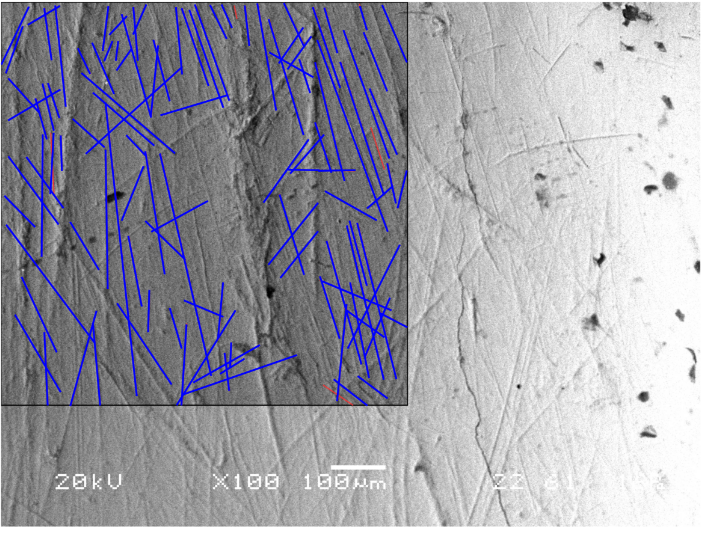
\includegraphics[width=.9\textwidth]{prueba4Detec}
	\caption{Estrías pintadas por la aplicacion prueba 4.}\label{fig:calcp4}
	\end{subfigure}%
	\caption{Imágenes prueba 4}
	\label{fig:p4}

\end{figure}

\apendice{Documentación de usuario}

\section{Introducción}
En esta sección, nos vamos a centrar en explicar y mostrar paso a paso, como un usuario puede llegar a usar esta aplicación de forma intuitiva y sencilla.
\section{Requisitos de usuarios}
Para que un usuario pueda ejecutar y usar nuestra aplicación, deberá tener instalado Python 3.5 en su maquina, aunque para facilitar al usuario no tener que saber como descargar las librerías o dependencias, hemos implementado un script que funcionara teniendo instalado Miniconda para Python 3.5, explicaremos su uso en la instalación.

\begin{itemize}
	\item Tener una distribución Windows instalada.

	\item Python 3.5: Para poder ejecutar necesitaremos tener Python 3.5.
	\begin{itemize}
		\item Miniconda para Python 3.5:
		
		Se puede descargar a través del siguiente enlace \url{http://conda.pydata.org/miniconda.html} y siguiendo las instrucciones a traves de este otro enlace \url{http://conda.pydata.org/docs/install/quick.html#windows-miniconda-install}.		
		
		Es una distribución que incluye Python y facilita el uso de este lenguaje y la instalación de multitud de librerías.
		
		Sera necesario tenerlo instalado en la carpeta principal de nuestro usuario C:\textbackslash Users\textbackslash NombreTuUsuario
	\end{itemize}
	
	\item Tener el proyecto descargado o clonado con los fuentes:
	
	Se puede descargar a través del siguiente enlace \url{https://github.com/Itg0001/TFG_DietaPorDientes.git}

\end{itemize}

\section{Instalación}

Una vez que tengamos Miniconda para Python 3.5 y el proyecto descargado o clonado podremos proceder a la instalación del mismo, siguiendo los pasos descritos a continuación:

\begin{itemize}
	\item Primero si hemos descargado el proyecto lo tendremos en formato .zip deberemos descomprimirlo en la carpeta deseada.
	
	\item Una vez descomprimido dentro del fichero del proyecto estará ubicado un ejecutable para Windows .bat llamado <<EjecutarGui.bat>>.
	
	Procederemos a hacer doble clic sobre este fichero ejecutable y se abrirá una terminal, la primera vez que lo hagamos este proceso tardara un rato, porque descarga las librerías necesarias para la ejecución del mismo.
	
	\item Una vez terminado el proceso anterior, se abrirá la aplicación.
\end{itemize}

\subsection{Cuando algo falla}
En caso de que al instalar o descargar los paquetes salta algún error esto se deberá a que se habrá perdido la conexión a Internet y no puede descargar los paquetes necesarios.
Para solucionarlo volvemos a ejecutar y comenzara donde se quedo al caerse la red. No perdemos el tiempo usado hasta ese momento.

Otro fallo común es que no se haya instalado la distribución de Miniconda sobre el directorio indicado: C:\textbackslash Users\textbackslash NombreTuUsuario.
Para solucionar este problema deberemos instalarlo sobre este directorio.

En caso de que surja algún otro problema contactar con el desarrollador a través del siguiente EMAIL: itg0001\makeatletter @ alu.ubu.es 

\section{Manual del usuario}

Una vez tengamos todo bien configurado y la aplicación ejecute correctamente deberíamos tener esta ventana inicial.

\begin{figure}[h]
\centering
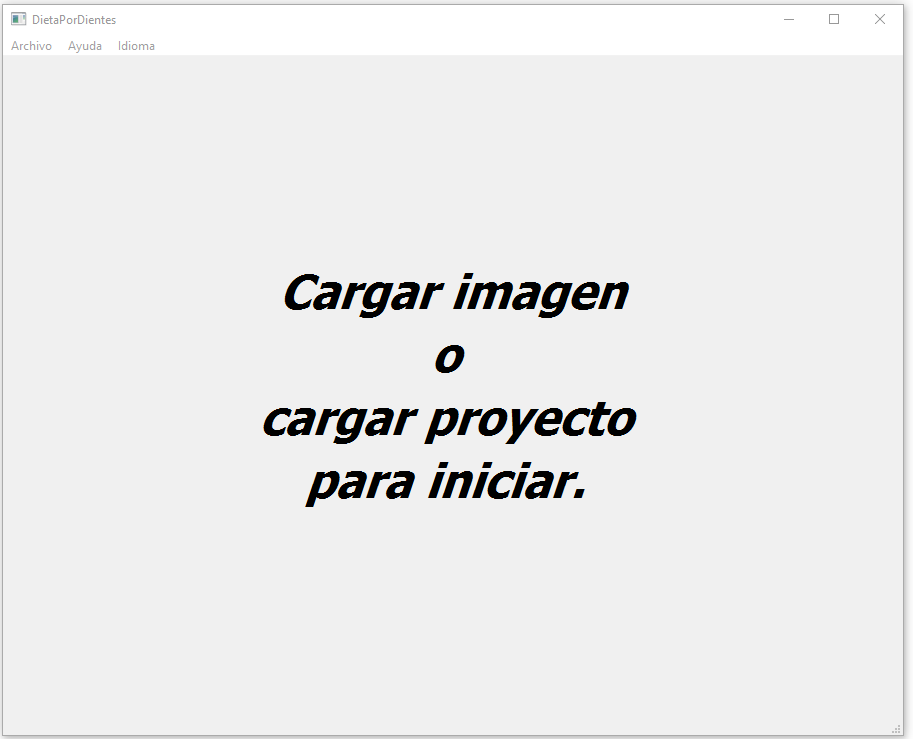
\includegraphics[width=.99\textwidth]{VentanaInicial}
\caption{Ventana inicial de la aplicación}
\label{fig:E.1}
\end{figure}
Una vez llegados a este punto tendremos varias opciones para editar o calculas las estrías de una imagen, dependiendo si esta en blanco o ya pintada tendremos las siguientes opciones:

\begin{itemize}
	\item Abrir imagen \ref{modo:1}:

	\item Cargar proyecto \ref{modo:2}:
	
\end{itemize}


\label{modo:1}
\subsection{Abrir imagen}
En esta sección se explicara como cargar una imagen en nuestra aplicación, para empezar un proyecto desde cero.

Deberemos seleccionar la opción de Archivo  $>$ Nuevo Proyecto. Como se puede ver en la imagen \ref{fig:abrirPro}

\begin{figure}[h]
\centering
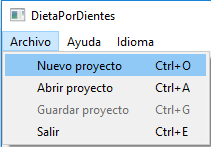
\includegraphics[width=.50\textwidth]{AbrirImagen}
\caption{Opción para cargar una imagen}
\label{fig:abrirPro}
\end{figure}

Una vez que clicamos en este punto se nos muestra una ventana de elegir ficheros en el cual debemos explorar hasta la carpeta donde estén las imágenes que queremos analizar. Como podemos observar en la figura \ref{fig:abrirPaso2}

\begin{figure}[h]
\centering
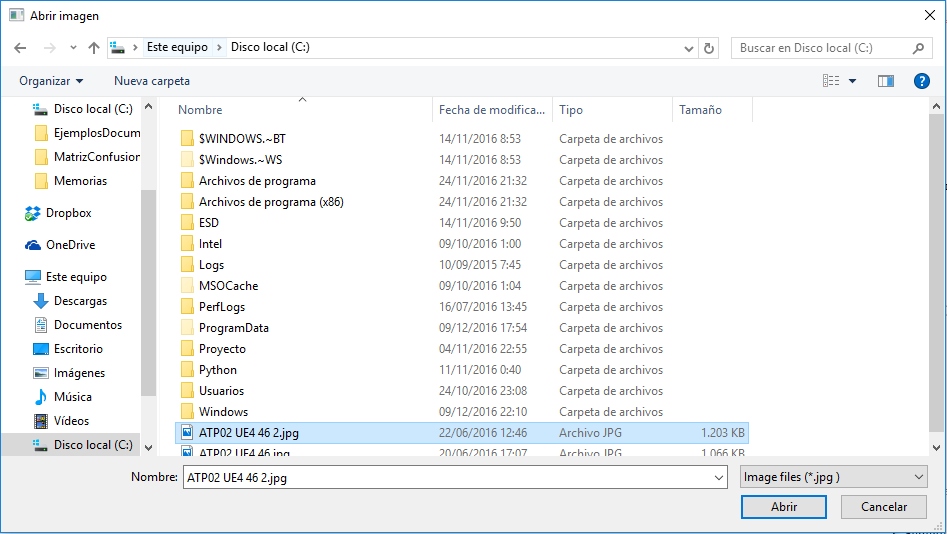
\includegraphics[width=.99\textwidth]{AbrirPaso2}
\caption{Seleccionador de ficheros}
\label{fig:abrirPaso2}
\end{figure}

Una vez seleccionado deberemos dar a aceptar si hemos seleccionado la imagen que queremos evaluar.
Dependiendo de la imagen que hemos abierto pueden pasar dos cosas, uno \ref{fig:opcion1}, que la imagen abierta este pintada, dos \ref{fig:opcion2}, que la imagen abierta no este pintada. Dependiendo de esto tendremos estas dos ventanas, como se muestra en la figura.


\begin{figure}
	\begin{subfigure}[c]{.5\linewidth}
	\centering\large 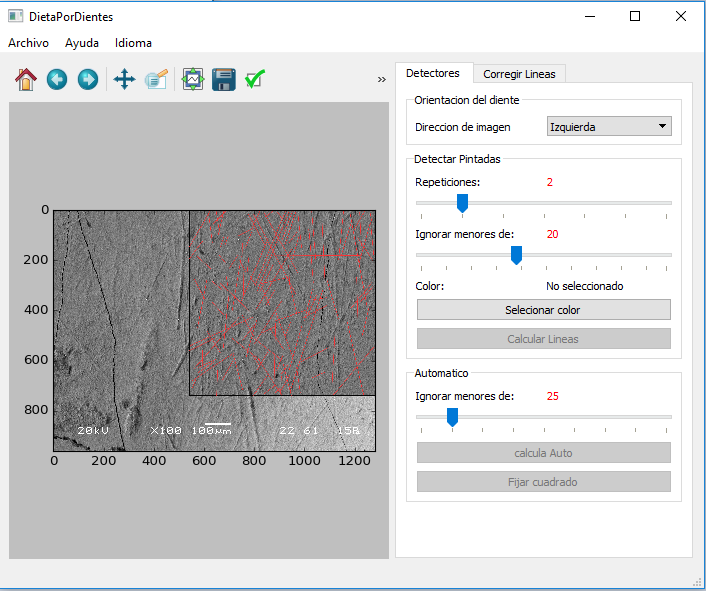
\includegraphics[width=.9\textwidth]{opcion1}
	\caption{Opcion con lineas pintadas.}\label{fig:opcion1}
	\end{subfigure}%
	\begin{subfigure}[c]{.5\linewidth}
	\centering\large 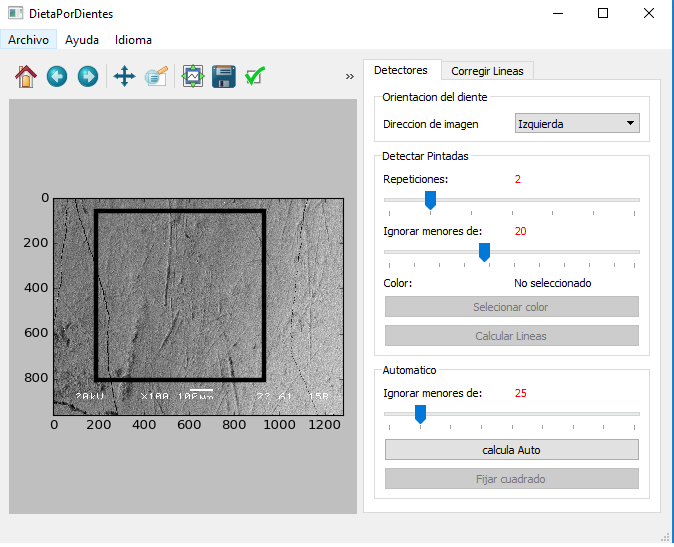
\includegraphics[width=.9\textwidth]{opcion2}
	\caption{Opcion con lineas sin pintar.}\label{fig:opcion2}
	\end{subfigure}%
\end{figure}




\label{modo:2}
\subsection{Cargar proyecto}
En esta sección se explicara como cargar un proyecto en nuestra aplicación, para continuar un proyecto ya empezado.

Deberemos seleccionar la opción de Archivo  $>$ Abrir Proyecto. Como se puede ver en la figura \ref{fig:cargarPro}


\begin{figure}[h]
\centering
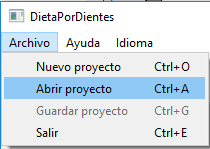
\includegraphics[width=.50\textwidth]{CargarProyecto}
\caption{Opción para abrir un proyecto.}
\label{fig:cargarPro}
\end{figure}

Una vez que hacemos clic sobre la opción anteriormente mencionada ahora debemos seleccionar la carpeta donde estará contenido todos los ficheros del proyecto, como podemos observar en la siguiente figura \ref{fig:selecCargarPro}. y una vez seleccionado el directorio que contiene los ficheros del proyecto damos a <<Abrir carpeta>> para cargar el proyecto. 



\begin{figure}[h]
\centering
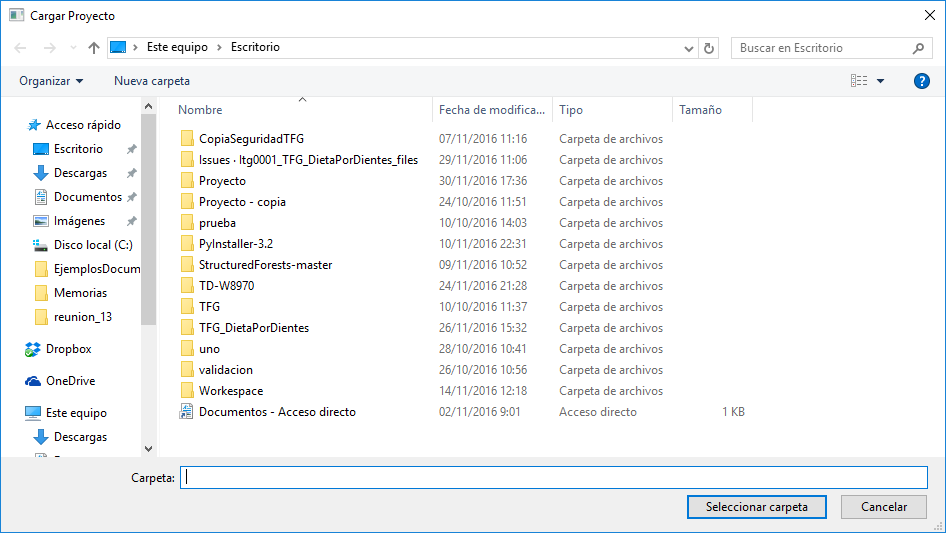
\includegraphics[width=.99\textwidth]{selecCargarPro}
\caption{Opción para abrir un proyecto.}
\label{fig:selecCargarPro}
\end{figure}

Una vez abierto el proyecto tendremos la imagen en blanco y negro junto con sus estrías guardadas que estarán pintadas sobre la imagen, como podemos observar en la figura \ref{fig:proyectoAbierto}.


\begin{figure}[h]
\centering
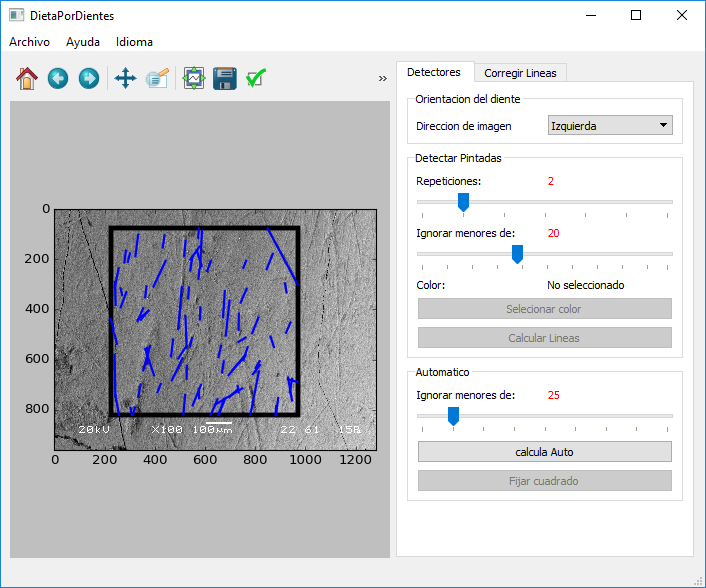
\includegraphics[width=.99\textwidth]{proyectoAbierto}
\caption{Como se muestra un proyecto cargado o abierto.}
\label{fig:proyectoAbierto}
\end{figure}

\label{modo:idioma}
\subsection{Cambiar idioma}
Para cambiar el idioma de la aplicación deberemos seleccionar en el menú principal Idioma $>$ Una de las dos opciones, como podemos observar en la figura \ref{fig:camb}, hemos optado por cambiar el idioma de la aplicación y que perduren los cambios realizados en el fichero de configuración por lo que nos va a pedir reiniciar la aplicación, si tenemos algo abierto nos preguntara si queremos guardar los cambios o no.

\begin{figure}[h]
\centering
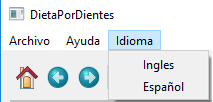
\includegraphics[width=.55\textwidth]{CambiarIdioma}
\caption{Como cambiar el idioma.}
\label{fig:camb}
\end{figure}

\subsection{Modo semi-automático para lineas pintadas}

Este modo solamente podrá ser usado cuando dispongamos de una imagen que tenga las estrías pintadas sobre ella y estas estén contenidas dentro de un cuadrado que delimite su área, como podemos observar en la figura \ref{fig:semiAutoCorrecto}.



\begin{figure}[h]
\centering
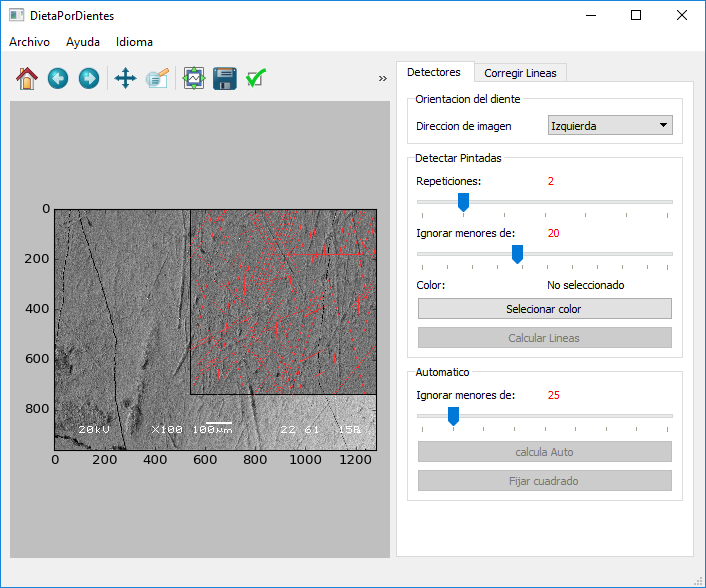
\includegraphics[width=.99\textwidth]{semiAutoCorrecto}
\caption{Imagen valida para detección de estrías modo semiautomático.}
\label{fig:semiAutoCorrecto}
\end{figure}

Una vez que tengamos una imagen con las estrías pintadas cargada y valida como mostramos en la figura, procederemos a seleccionar su orientación, como muestra en la siguiente figura \ref{fig:selOrientacion}.

\begin{figure}[h]
\centering
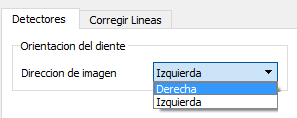
\includegraphics[width=.55\textwidth]{selOrientacion}
\caption{Selección de la orientación de la imagen.}
\label{fig:selOrientacion}
\end{figure}

A continuación deberemos seleccionar tanto el numero de repeticiones del algoritmo para la obtención de los segmentos pintados <<Cuanto mayor número de ellos mas tiempo tardara>>, la longitud mínima que debe ignorar el algoritmo para no detectar segmentos muy pequeños. Como podemos observar en la figura \ref{fig:opcionesAlg}.

\begin{figure}[h]
\centering
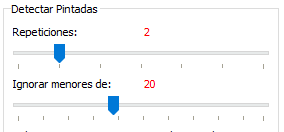
\includegraphics[width=.55\textwidth]{opcionesAlg}
\caption{Selección de las opciones disponibles para este modo.}
\label{fig:opcionesAlg}
\end{figure}

Finalmente para nos quedaría la opción mas importante que sin ella el algoritmo no podrá ser ejecutado. Es seleccionar el color del que estén pintadas las lineas, para ello deberemos clicar sobre el botón <<Seleccionar color>>, como podemos observar en la figura \ref{fig:selecionarColorP1} y después de clicar sobre el este se desactivara como podemos observar en la figura \ref{fig:selecionarColorP2}.
Las estrías pintadas aveces pueden ser muy finas y no seremos capaces de clicar sobre esos pixeles por lo que en este caso deberemos ampliar la imagen en una región que contenga estrías pintadas, para ampliar debemos seleccionar el botón de ampliar y dibujar un rectángulo sobre la imagen con el clic derecho pulsado,como podemos observar en la figura \ref{fig:selecionarColorP3}.
Una vez seleccionado el color correctamente este pintada el label de color actual y también se activara el botón de calcular las lineas, como podemos observar en la figura \ref{fig:selecionarColorP4}.



\begin{figure}
	\begin{subfigure}[c]{.5\linewidth}
	\centering\large 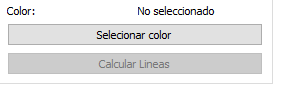
\includegraphics[width=.9\textwidth]{selecionarColorP1}
	\caption{Selección del color en el que estén las estrías pintadas.}\label{fig:selecionarColorP1}
	\end{subfigure}%
	\begin{subfigure}[c]{.5\linewidth}
	\centering\large 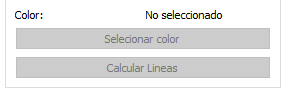
\includegraphics[width=.9\textwidth]{selecionarColorP2}
	\caption{Después de clicar sobre el.}
	\label{fig:selecionarColorP2}
	\end{subfigure}%
	
	\begin{subfigure}[c]{.5\linewidth}
	\centering\large \includegraphics[width=.9\textwidth]{selecionarColorP2}
	\caption{Ampliar región.}
	\label{fig:selecionarColorP3}
	\end{subfigure}%
	\begin{subfigure}[c]{.5\linewidth}
	\centering\large \includegraphics[width=.9\textwidth]{selecionarColorP4}
	\caption{Después de seleccionar correctamente el color.}
	\label{fig:selecionarColorP4}
	\end{subfigure}%
\end{figure}

Para finalizar una vez que cliquemos en el botón de calcular lineas ya podremos añadir estrías nuevas, eliminar algunos segmentos, borrar todos o guardar los datos del proyecto para calcular las estadísticas de las estrías.


\subsection{Modo manual}
Después de cargar una imagen ya sea pintada o sin pintar deberemos abrir una imagen como indica el apartado \ref{modo:1} o abrir un proyecto tal y como indican el apartado \ref{modo:2}.
Una vez que tengamos la imagen o el proyecto cargado podremos pintar nuevas estrías en la imagen siguiendo los siguientes pasos.

\begin{itemize}
\item Pulsaremos el botón de corregir lineas, como muestra la siguiente figura \ref{fig:CorregirPaso1}.

\item Una vez pulsado deberemos seleccionar dos puntos, uno el inicio y el segundo, el final del segmento que queremos añadir. 
Dentro del recuadro de la región factible que esta delimitada por un recuadro negro, como se muestra en las figuras \ref{fig:punto1} y \ref{fig:punto2}, ahora solo nos quedara añadir el segmento a la tabla como muestra la figura \ref{fig:anadirsegment}.
\end{itemize}

\begin{figure}
	\begin{subfigure}[c]{.5\linewidth}
	\centering\large \includegraphics[width=.9\textwidth]{CorregirPaso1}
	\caption{Activar el modo de corregir o añadir un segmento.}\label{fig:CorregirPaso1}
	\end{subfigure}%
	\begin{subfigure}[c]{.5\linewidth}
	\centering\large \includegraphics[width=.9\textwidth]{punto1}
	\caption{Primer punto seleccionado.}\label{fig:punto1}
	\end{subfigure}%
	
	\begin{subfigure}[c]{.5\linewidth}
	\centering\large \includegraphics[width=.9\textwidth]{punto2}
	\caption{Segundo punto seleccionado.}\label{fig:punto2}
	\end{subfigure}%
	\begin{subfigure}[c]{.5\linewidth}
	\centering\large \includegraphics[width=.9\textwidth]{anadirsegment}
	\caption{Añadir segmento.}\label{fig:anadirsegment}
	\end{subfigure}%
\end{figure}

	
Para los demás pasos no hace falta explicación ya que sus respectivos botones dicen claramente que funciones desempeñan.	
	
\subsection{Modo automático}
Después de cargar una imagen sin pintar deberemos abrir una imagen como indica el apartado \ref{modo:1} o abrir un proyecto tal y como indica el apartado \ref{modo:2}.

Una vez que tengamos la imagen o el proyecto cargado, podremos configurar el modo automático, lo primero sera asignar la orientación de la imagen, como podemos ver en la figura \ref{fig:selOrientacion}, también deberemos seleccionar la longitud mínima de corte que ignorara el algoritmo automático, como podemos observar en la figura \ref{fig:selTam}.

\begin{figure}[h]
\centering
\includegraphics[width=.55\textwidth]{selTam}
\caption{Selección de la longitud mínima de corte.}
\label{fig:selTam}
\end{figure}

Una vez seleccionado el tamaño mínimo de corte podremos ejecutar el algoritmo clicando el botón de calar automático obteniendo el resultado mostrado en la figura \ref{fig:CalculadasAuto} y podremos mover el recuadro del área con el que nos queremos quedar a la región de interés que consideremos apropiada.

\begin{figure}[h]
\centering
\includegraphics[width=.55\textwidth]{CalculadasAuto}
\caption{Selección de la longitud mínima de corte.}
\label{fig:CalculadasAuto}
\end{figure}

una vez que la situemos donde mayor densidad de estrías haya detectado, la fijaremos e ignorara las que se queden por fuera de la región, como podemos observar en la figura \ref{fig:automati}.

\begin{figure}[h]
\centering
\includegraphics[width=.55\textwidth]{automati}
\caption{Selección de la longitud mínima de corte.}
\label{fig:automati}
\end{figure}

Pasado este punto en la pestaña de corregir lineas quedaran añadidas todas aquellas que ha detectado el algoritmo y hemos encuadrado en la región factible, de estas lineas podremos obtener tanto estadísticas como un proyecto para editar mas adelante. Guardando el proyecto con el botón para dicha función.

\subsection{Guardar proyecto}

En este apartado vamos a explicar como guardar un proyecto una vez que hayamos abierto o cargado una imagen, calculado las estrías con el modo semiautomático o por el automático, y la tabla este rellenada con estas. 
Si el proyecto es cargado de uno ya existente, no tener abiertas las estadísticas en Excel porque sino no funcionara la operación de guardar, esto sera transparente al usuario porque dejara los ficheros como estaban antes, no los modificara, e informara al usuario de que no han sido guardados. 

Podemos usar tanto el botón de guardar que aparece en la pestaña dos \ref{fig:BotonGuarPesta} como el botón del menú principal que aparece en la figura \ref{fig:BotonGuar}

\begin{figure}
	\begin{subfigure}[c]{.5\linewidth}
	\centering\large \includegraphics[width=.9\textwidth]{BotonGuarPesta}
	\caption{Boton de guardar en la pestaña dos.}\label{fig:BotonGuarPesta}
	\end{subfigure}%
	\begin{subfigure}[c]{.5\linewidth}
	\centering\large \includegraphics[width=.9\textwidth]{BotonGuar}
	\caption{Boton de guardar en el menu principal.}\label{fig:BotonGuar}
	\end{subfigure}%
\end{figure}

\apendice{Procesado automático de la imagen}
\label{anexo:F}
\section{Introducción}
En este apartado vamos a explicar lo que hemos investigado sobre la detección de bordes para el modo automático.

Esto lo vamos afrontar desde dos puntos de vista, el primero será por el procesado de imágenes, esto consistirá en obtener una mascara con los bordes de la imagen usando un kernel conocido y observar si los resultados nos muestran algún resultado factible.
Como segunda opción vamos a intentar ejecutar algoritmos de Deep Learning para ver si mejora el resultado usando estos algoritmos.

Para entender este anexo y este procesado, por lo menos es necesario haberse leído los conceptos teóricos y herramientas mencionadas en la memoria ya que no se ha duplicado dicha información en varios sitios.

\section{Extracción de bordes mediante procesado de imagen}
Esta sección consistirá, partiendo de una imagen en extraer las características, en este caso será la detección de los bordes contenidos, se corresponderán con las estrías que queremos detectar. Lo vamos a detectar a partir de los métodos explicados a continuación. 

A todas las imágenes se las va a aplicar un proceso de convolución, con el Kernel \cite{wiki:kernels} específico en cada caso.

Una convolución es una operación matemática, que no es la multiplicación de matrices tradicional, es el proceso de agregar cada porción de la imagen a sus vecinos locales ponderado por el Kernel. 
Este proceso no solo vale para detectar bordes, tiene estas otras aplicaciones.
\begin{itemize}
\item Detección de bordes: Detectar los puntos donde acaba un objeto y empieza otro, también las aristas o bordes de las imágenes.
\item Desenfoques y difuminado: Desenfocar o difuminar la imagen a partir de hacer la operación de convolución con una máscara diseñada para ello.
\item Eliminar ruido: Sirve para moderar los valores de la imagen  y hacer que estén mas centrados en un rango y así eliminar el ruido aleatorio. 
\end{itemize}

\subsection{Laplace:}
Esta función busca bordes usando el operador de Laplace \cite{wiki:Laplace}. En nuestro caso de tamaño 3 (ya que se puede especificar el tamaño).
Se ilustra el Kernel de Laplace en la figura~\ref{F_k1}.


Observaciones:
Como se ilustra en la figura~\ref{fig:1.1.1}, no es un método válido para nuestro propósito, porque no detecta los bordes, simplemente deja algunas partes difuminadas, pero nada sobre lo que podamos trabajar para obtener la imagen binarizada. Por lo que no vamos a continuar usándolo.

\subsection{Prewitt:}

Encuentra los bordes usando la transformada de Prewitt \cite{wiki:Prewitt}.

Se ilustra el Kernel de Prewitt en la figura~\ref{F_k2}.



Observaciones:
Como podemos ver las grietas, en la figura~\ref{fig:1.1.2}, las detecta bien pero las estrías de dieta son siluetas muy tenues y contiene mucho ruido.


\subsection{Scharr:}
Con este método encontramos los bordes usando la transformada de Scharr \cite{wiki:Scharr}.
Se ilustra el Kernel de Scharr en la figura~\ref{F_k3} todo ello partido de 16 y para las verticales es la matriz transpuesta. 




Observaciones:
Como podemos ver en la figura~\ref{fig:1.1.3}, las estrías de dieta son muy tenues pero ligeramente mejores que en la anterior, tampoco demasiado pero ligeramente, el método es algo más rápido también pero no obtenemos algo tangible, en cuanto  a bordes detectados ya que se muestran de forma muy tenue y no podrán ser extraídos en la binarización necesitaríamos mayor diferencia, entre el fondo el y borde.




\subsection{Sobel:}
Este método busca bordes usando la transformada de Sobel \cite{wiki:Sobel}.

Se ilustra el Kernel de Sobel en la figura~\ref{F_k4}.


El kernel de Sobel, partido de 4 para los bordes horizontales.
Para los bordes verticales, es el kernel de Sobel, partido de 4 y transpuesto. 

Observaciones: 
Con este método tal y como podemos ver en la figura~\ref{fig:1.1.4}, crea más ruido que los anteriores pero también podemos vislumbrar las siluetas de las estrías de dieta.


\subsection{Roberts:}

Esta función encuentra los bordes usando la operación cruzada de Robert \cite{wiki:Roberts}.

Se ilustra el Kernel de Roberts en la figura~\ref{F_k5}.




Observaciones:
Como podemos ver en la figura~\ref{fig:1.1.5}, este método produce mucho ruido y las estrías son líneas demasiado tenues.

\subsection{Kirsch:}
Esta función encuentra los bordes usando el kernel de Kirsch \cite{wiki:Kirsch}. Para cada dirección.
No estaba implementado en Skimage por lo que he implementado el método.
Como podemos ver en las figuras~\ref{F_k6_1},~\ref{F_k6_2},~\ref{F_k6_3} y~\ref{F_k6_4}, están los kernel para los bordes Horizontal, vertical diagonal ascendente y diagonal descendente.
\begin{table}[!htb]

	\begin{minipage}{.5\linewidth}
		\centering
		\caption{Kernel g1}
		\label{F_k6_1}
		\begin{tabular}{|r|r|r|}
			\hline
			5  & 5  & 5  \\ \hline
			-3 & 0  & -3 \\ \hline
			-3 & -3 & -3 \\ \hline
		\end{tabular}
    \end{minipage}%
	\begin{minipage}{.5\linewidth}
		\centering
		\caption{Kernel g2}
		\label{F_k6_2}
		\begin{tabular}{|r|r|r|}
			\hline
			5  & 5  & -3  \\ \hline
			5 & 0  & -3 \\ \hline
			-3 & -3 & -3 \\ \hline
		\end{tabular}
    \end{minipage}%


	\begin{minipage}{.5\linewidth}
		\centering
		\caption{Kernel g3}
		\label{F_k6_3}
		\begin{tabular}{|r|r|r|}
			\hline
			5  & -3 & -3  \\ \hline
			5 & 0  & -3 \\ \hline
			5 & -3 & -3 \\ \hline
		\end{tabular}
    \end{minipage}%	
	\begin{minipage}{.5\linewidth}
		\centering
		\caption{Kernel g4}
		\label{F_k6_4}
		\begin{tabular}{|r|r|r|}
			\hline
			-3  & -3 & -3  \\ \hline
			5 & 0  & -3 \\ \hline
			5 & 5 & -3 \\ \hline
		\end{tabular}
    \end{minipage}%
    \caption{Distintos kernels de Kirsch}
\end{table}

Observaciones:
Como podemos observar en la figura~\ref{fig:1.1.9}.
Este método produce mucho ruido y las estrías son líneas demasiado tenues.
No obstante de los métodos hasta ahora usados es en el que mas aprecian.


\begin{table}[]

	\begin{minipage}{.5\linewidth}
		\centering
		\caption{Kernel Laplace}
		\label{F_k1}
		\begin{tabular}{|r|r|r|}
			\hline
			0 & 1  & 0 \\ \hline
			1 & -4 & 1 \\ \hline
			0 & 1  & 0 \\ \hline
		\end{tabular}
    \end{minipage}%
	\begin{minipage}{.5\linewidth}
		\centering
		\caption{Kernel Prewitt}
		\label{F_k2}
		\begin{tabular}{|r|r|r|}
			\hline
			1  & 1   & 1 \\ \hline
			0  & 0   & 0 \\ \hline
			-1 & -1  & -1 \\ \hline
		\end{tabular}
    \end{minipage}%
    \\

	\begin{minipage}{.5\linewidth}
		\centering
		\caption{Kernel HScharr}
		\label{F_k3}
		\begin{tabular}{|r|r|r|}
			\hline
			3  & 10  & 3 \\ \hline
			0  & 0   & 0 \\ \hline
			-3 & -10 & -3 \\ \hline
		\end{tabular}
    \end{minipage}%
	\begin{minipage}{.5\linewidth}
		\centering
		\caption{Kernel HSobel}
		\label{F_k4}
		\begin{tabular}{|r|r|r|}
			\hline
			1  & 2  & 1 \\ \hline
			0  & 0  & 0 \\ \hline
			-1 & -2 & -1 \\ \hline
		\end{tabular}
    \end{minipage}%
    
	\begin{minipage}{.5\linewidth}
		\centering
		\caption{Kernel Roberts}
		\label{F_k5}
		\begin{tabular}{|r|r|}
			\hline
			0  & 1 \\ \hline
			-1 & 0 \\ \hline
		\end{tabular}
    \end{minipage}%
	\caption{Kernels de los métodos analizados.}
\end{table}


\subsection{Autovectores matriz Hessiana:}
Este método consiste en obtener la matriz hessiana \cite{wiki:Hessiana} y después sus autovectores, esto nos devuelve dos matrices la matriz i1 es la matriz con el autovector más largo y la i2 es la matriz con autovector más corto.



Observaciones: 
Antes de aplicar el método, podemos leer en la documentación de Skimage, que es apropiado para detectar bordes continuos, entre otras formas, por lo que podemos pensar que en nuestro caso, cumple los requisitos para una buena detección ya que estos también son continuos. 
Como podemos observar en la figura~\ref{fig:1.1.6} en escala de grises del autovector de los valores más largos las siluetas de las estrías de dieta son las que más se remarcan sobre un tenue fondo gris pero pudiendo ser observadas por lo que este podría ser un punto de partida.



\subsection{Canny:}

\subsubsection{Eliminando ruido:}
Primero, obtener los bordes, llamar a una función que elimina el ruido y después al detector de bordes Canny \cite{wiki:Canny}, para obtener los bordes.
Para los parámetros usados en la función de Canny utilizaremos:
\begin{itemize}
	\item Sigma: Un valor intermedio de 1.4.
	Este parámetro afecta a la desviación estándar del filtro Gausiano.
	\item Umbral mínimo: Un valor muy bajo.
	Este parámetro nos indica el valor mínimo para ser considerado un borde.
	\item Umbral Máximo: Un valor bajo pero mayor que el umbral mínimo.
	Este parámetro nos indica el valor máximo para ser considerado un borde.
\end{itemize}
Gracias a estos parámetros usados obtenemos una imagen resaltando algunos bordes pero no todo los que queremos ya que no están demasiado marcados.




Observaciones:
Desde esta figura~\ref{fig:1.1.7} con bastante ruido ya podemos observar que las más marcadas son detectadas pero no se consiguen diferenciar demasiado bien, pero en comparación con los demás métodos tiene de las mejores salidas aun no siendo buena de ir en esta línea tendiéramos que usar esto.

\subsubsection{Modificando parámetros Canny:}

La segunda opción ha sido usar un detector de bordes Canny solamente modificando sus parámetros pero en esta opción los valores de los umbrales deben ir sin normalizar entre 0 y 1, sino entre 0 y 255.


Observaciones:
La figura~\ref{fig:1.1.8} detecta menos ruido que con la otra tentativa pero sigue siendo deficiente en cuanto a las líneas ya que aparte de detectar pocas detecta las que realmente no son estrías de dieta. Pero de ir en alguna línea sería por este camino.



\subsection{Gabor:}

Gabor \cite{wiki:Gabor} es un filtro linear con un kernel gausiano  que es modulado por un onda sinusoidal plana. Principalmente se usa en visión artificial de clasificación y detección de bordes.
Obtenemos un par de imágenes.



Observaciones:
Como podemos observar en la imagen usando Gabor con filtro imaginario~\ref{fig:1.1.10}.
Como podemos observar en la imagen usando Gabor con filtro real~\ref{fig:1.1.11}.
Este método lo he probado porque en la obtención, de las líneas correspondientes a vasos sanguíneos en los ojos <<blood vessels detection \cite{Xu2010}>> es lo que se usa para ello pero al no ser líneas continuas y no seguir un patrón no he conseguido buenos resultados. En el filtro real no es tan malo pero en el filtro imaginario es ruido puro.
\subsection{Comparativa Filtros}
Como podemos ver en la figura~\ref{fig:1.1} hemos usado casi todos los filtros conocidos para hacer esta comparativa, a simple vista ninguno de los métodos mencionados o probados no parece que funcione, ya que el problema no es fácil.
Manualmente no observamos algunas de las estrías que los expertos marcan por lo tanto, detectar algunas sera algo efectivo.

Pero dentro de la comparativa la que mejor detecta algunos de los bordes parece el método de la matriz Hessiana con autovectores largos. Aunque en la imagen se presenta poca diferencia entre fondo y las estrías por lo que nos centraremos en ese procesado haber si conseguimos diferenciarlo y extraer las características.

\subsection{Procesado:}
Partiendo del análisis anterior vamos a juntar los mejores resultados y añadir pasos adicionales para obtener la máscara binaria que mas podamos ajustar a nuestras necesidades.

La detección de los bordes en la imagen es solo uno de los pasos en nuestro algoritmo, este se compone por una serie de pasos divididos en tres categorías, preprocesado para mejorar la calidad de la imagen, Detección de bordes y postprocesado de la imagen de bordes. Todos los pasos del algoritmo se muestran en la figura~\ref{fig:2.1}.

\begin{itemize}
\item Preprocesado:
	\begin{itemize}
		\item Ecualizar la imagen original~\ref{fig:2.1.1}, consistirá en extender el histograma de la imagen original para que no este centrado en un rango pequeño como podemos observar en su histograma~\ref{fig:2.1.2}, pasado este paso obtendremos la imagen ecualizada~\ref{fig:2.1.3}.
Así conseguimos que su histograma~\ref{fig:2.1.4} este mas repartido por toda la gama de grises y no centrado en un pequeño rango.
	\end{itemize}
	
\item Detección de bordes:
	\begin{itemize}
		\item Autovectores de la Hessiana~\ref{fig:2.1.5}:
Para detectar los bordes utilizaremos el método antes mencionado de la matriz Hessiana del cual elegiremos solo los largos, ya que los autovectores pueden ser los cortos o los largos. 
		\item Sustraemos el fondo a la figura~\ref{fig:2.1.6}:
Como la imagen no tiene de nuevo demasiada diferencia entre el fondo y los bordes, sustraeremos el fundo, para quedarnos únicamente con las estrías detectadas, al tener ruido aparte de los elementos buscados, tendremos que eliminar dicho ruido mas adelante.
		\item Binarizamos la figura~\ref{fig:2.1.7}:
Como la imagen después de sustraer el fondo no es binaria, cualidad necesaria para ser una máscara.
Hay que aplicar un threshold o umbral para pasar a blanco o negro, binarizar, es decir los pixeles que no pasen el umbral serán negros y los que lo pasen formaran parte de los elementos que queremos detectar y seran blancos.
Entonces la imagen quedara binarizada.
	\end{itemize}
	
\item Postprocesado de la imagen y bordes:
	\begin{itemize}
		\item Eliminamos el ruido~\ref{fig:2.1.8}:
El paso anterior, en estas condiciones de trabajo genera mucho ruido, por lo que tendremos que intentar reducirlo y para ello eliminamos los trozos que son pequeños, ya que el ruido parece ser aleatorio de fragmentos muy pequeños, esto elimina la mayoría de los puntos de ruido.
		\item Erosionar con operador diamante~\ref{fig:2.1.9}:
Para suavizar la imagen y evitar que queden líneas finas a modo de antenas, erosionamos la imagen con un operador estructurante en forma de diamante, así conseguimos que pase por la mayoría de las figuras.
		\item Esqueletonizar la imagen~\ref{fig:2.1.10}:
Una vez tengamos la imagen sin tanto ruido, reducimos el grosor de las líneas para que la función de Hough funcione, así nos detecta las líneas que corresponden a esta máscara binaria.
		\item Eliminar mas ruido~\ref{fig:2.1.11}:
Este paso anterior vuelve a generar ruido porque algunos trozos se dividen en pequeños segmentos y con la segunda reducción de ruido conseguimos hacerlos desaparecer y quedarnos con las líneas grandes.
		\item Detectar los segmentos~\ref{fig:2.1.12}:
Una vez que tenemos todos los segmentos detectados mediante Hough, que se corresponden con las líneas que hay en la imagen, tenemos que unir los que sean contiguos y muy cercanos, para formar segmentos mas grandes.
		\item Unir segmentos cercanos~\ref{fig:2.1.13}:
Para este paso vamos a usar lo mismo que hemos utilizado dentro de la parte, detección de las líneas pintadas.
La imágenes tienen mucho ruido y aunque hemos conseguido procesar y reducirlo, aun no vamos a detectar un alto por ciento de las estrías.
	\end{itemize}

\end{itemize}



\begin{figure}
	\begin{subfigure}[c]{.33\linewidth}
	\centering\large \includegraphics[width=.9\textwidth]{Laplace}
	\caption{Bordes usando Laplace}\label{fig:1.1.1}
	\end{subfigure}%
	\begin{subfigure}[c]{.33\linewidth}
	\centering\large \includegraphics[width=.9\textwidth]{Prewitt}
	\caption{Bordes usando Prewitt}\label{fig:1.1.2}
	\end{subfigure}%
	\begin{subfigure}[c]{.33\linewidth}
	\centering\large \includegraphics[width=.9\textwidth]{Scharr}
	\caption{Bordes usando Scharr}\label{fig:1.1.3}
	\end{subfigure}%
		
	\begin{subfigure}[c]{.33\linewidth}
	\centering\large \includegraphics[width=.9\textwidth]{Sobel}
	\caption{Bordes usando Sobel}\label{fig:1.1.4}
	\end{subfigure}%
	\begin{subfigure}[c]{.33\linewidth}
	\centering\large \includegraphics[width=.9\textwidth]{Roberts}
	\caption{Bordes usando Roberts}\label{fig:1.1.5}
	\end{subfigure}%	
	\begin{subfigure}[c]{.33\linewidth}
	\centering\large \includegraphics[width=.9\textwidth]{HessianaAutoLargos}
	\caption{Bordes usando HessianaAutoLargos}\label{fig:1.1.6}
	\end{subfigure}%
	
	\begin{subfigure}[c]{.33\linewidth}
	\centering\large \includegraphics[width=.9\textwidth]{CannyP}
	\caption{Bordes usando CannyP}\label{fig:1.1.7}
	\end{subfigure}%
	\begin{subfigure}[c]{.33\linewidth}
	\centering\large \includegraphics[width=.9\textwidth]{Canny}
	\caption{Bordes usando Canny}\label{fig:1.1.8}
	\end{subfigure}%	
	\begin{subfigure}[c]{.33\linewidth}
	\centering\large \includegraphics[width=.9\textwidth]{Kirsch}
	\caption{Bordes usando Kirsch}\label{fig:1.1.9}
	\end{subfigure}	
	
	\begin{subfigure}[c]{.33\linewidth}
	\centering\large \includegraphics[width=.9\textwidth]{GaborI}
	\caption{Bordes usando Gabor filtro imaginario}\label{fig:1.1.10}
	\end{subfigure}%	
	\begin{subfigure}[c]{.33\linewidth}
	\centering\large \includegraphics[width=.9\textwidth]{GaborR}
	\caption{Bordes usando Gabor filtro real}\label{fig:1.1.11}
	\end{subfigure}

\caption{Resumen visual filtros usados.}\label{fig:1.1}
\end{figure}






\begin{figure}

	\begin{subfigure}[c]{.55\linewidth}
	\centering\large \includegraphics[width=.9\textwidth]{Imagen}
	\caption{Imagen original}\label{fig:2.1.1}
	\end{subfigure}%
	\begin{subfigure}[c]{.55\linewidth}
	\centering\large \includegraphics[width=.9\textwidth]{ImagenHist}
	\caption{Histograma imagen original}\label{fig:2.1.2}
	\end{subfigure}%
	
	\begin{subfigure}[c]{.55\linewidth}
	\centering\large \includegraphics[width=.9\textwidth]{Equalized}
	\caption{Imagen ecualizada}\label{fig:2.1.3}
	\end{subfigure}%	
	\begin{subfigure}[c]{.55\linewidth}
	\centering\large \includegraphics[width=.9\textwidth]{Histograma_Equali}
	\caption{Histograma imagen ecualizada}\label{fig:2.1.4}
	\end{subfigure}%
	\caption{Pasos del procesado parte uno.}\label{fig:2.1}

\end{figure}
 
	

\begin{figure}
	\begin{subfigure}[c]{.49\linewidth}
	\centering\large \includegraphics[width=.9\textwidth]{HessianaPaso2}
	\caption{Autovectores largos.}\label{fig:2.1.5}
	\end{subfigure}%
	\begin{subfigure}[c]{.49\linewidth}
	\centering\large \includegraphics[width=.9\textwidth]{HessianaPaso2MenosFOndo}
	\caption{Hessiana menos fondo.}\label{fig:2.1.6}
	\end{subfigure}%
	
	\begin{subfigure}[c]{.49\linewidth}
	\centering\large \includegraphics[width=.9\textwidth]{MenosFondoBinarizada}
	\caption{Binarizado.}\label{fig:2.1.7}
	\end{subfigure}%	
	\begin{subfigure}[c]{.49\linewidth}
	\centering\large \includegraphics[width=.9\textwidth]{BinarizadaSinRuido}
	\caption{Binarizada sin ruido.}\label{fig:2.1.8}
	\end{subfigure}%	
	
	\begin{subfigure}[c]{.49\linewidth}
	\centering\large \includegraphics[width=.9\textwidth]{SinRuidoErosionada}
	\caption{Erosionado.}\label{fig:2.1.9}
	\end{subfigure}%	
	\begin{subfigure}[c]{.49\linewidth}
	\centering\large \includegraphics[width=.9\textwidth]{ErosionadaEsqueletonizada}
	\caption{Esqueletonizado de la erosión.}\label{fig:2.1.10}
	\end{subfigure}%	
		
	\begin{subfigure}{.49\linewidth}
	\centering\large \includegraphics[width=.9\textwidth]{EsqueletonizadaSinRuido}
	\caption{Esqueletonizada sin ruido}\label{fig:2.1.11}
	\end{subfigure}%
	\caption{Pasos del procesado parte dos.}\label{fig:2.2}

\end{figure}

\begin{figure}

	\begin{subfigure}{.99\linewidth}
	\centering\large \includegraphics[width=.9\textwidth]{SegmentosSinUnir}
	\caption{Segmentos detectados}\label{fig:2.1.12}
	\end{subfigure}%
	
	\begin{subfigure}{.99\linewidth}
	\centering\large \includegraphics[width=.9\textwidth]{LineasReales}
	\caption{Segmentos reales}\label{fig:2.1.13}
	\end{subfigure}%
	
\caption{Pasos del procesado parte tres.}\label{fig:2.3}
\end{figure}

\section{Extracción de bordes mediante Deep Learning}


En esta sección vamos a intentar ejecutar algoritmos ya existentes de Deep Learning y si funcionan re-entrenarlos para que detecten los bordes en nuestras imágenes, pero para ello tendremos que probar todos lo posible y de los que funcionen y detecten decentemente probar que pasa si re-entrenamos para nuestras imágenes.

Algoritmos probados, en Matlab, en Python 3.5 y en Python 2.7:
\begin{itemize}
\item Tensorpack: Podemos encontrar el proyecto que contiene dicho algoritmo en GitHub atraves de este enlace: \url{https://github.com/ppwwyyxx/tensorpack}

\item Structured edge forest: Podemos encontrar el proyecto que contiene dicho algoritmo en GitHub atraves de este enlace: \url{https://github.com/pdollar/edges}

\item Sketch Tokens: Podemos encontrar el proyecto que contiene dicho algoritmo en GitHub atraves de este enlace: \url{https://github.com/gitlim/SketchTokens}

\item Oriented Edge Forests: Podemos encontrar el proyecto que contiene dicho algoritmo en GitHub atraves de este enlace: \url{https://github.com/RongchangZhao/oef}

\item Retina blood vessel: Podemos encontrar el proyecto que contiene dicho algoritmo en GitHub atraves de este enlace: \url{https://github.com/orobix/retina-unet}

\item StrudturedForest Python2: Podemos encontrar el proyecto que contiene dicho algoritmo en GitHub atraves de este enlace: \url{https://github.com/ArtanisCV/StructuredForests}
\end{itemize}

Una vez probados todos ellos, no hemos sido capaces de ejecutarlos, ya que por alguna razón en todos ellos, debía de faltar alguna clase, referencias o simplemente no estaban actualizados, en sus repositorios de GitHub.


\bibliographystyle{plain}
\bibliography{bibliografiaAnexos}

\end{document}